\documentclass[12pt, a4paper, ngerman, numbers=noenddot, twoside, open=right]{scrreprt}
\setkomafont{sectioning}{\normalfont\normalcolor\bfseries}

\usepackage{graphicx}
\usepackage{scrhack}
\usepackage{epsfig}
\usepackage[utf8]{inputenc}
\usepackage[ngerman]{babel}
\usepackage{amssymb}
\usepackage{dsfont}
\usepackage[printonlyused]{acronym}

\usepackage[colorlinks, pdfpagelabels, pdfstartview=FitH,
			bookmarksopen=true, bookmarksnumbered=true, linkcolor=black, plainpages=false, hypertexnames=false,
			citecolor=black, urlcolor=black]{hyperref}

\usepackage{float}
\usepackage{listings}
\usepackage{fancyhdr}
\usepackage{pdfpages}
\usepackage{todonotes}
\usepackage{enumitem}
\usepackage{longtable}
\usepackage{booktabs}
\usepackage{multirow}
\usepackage{lscape}
\usepackage{thesis}
\setcounter{secnumdepth}{3}

\fancyhf{}
\renewcommand{\chaptermark}[1]{\markboth{\chaptername\ \thechapter\ #1}{}}
\fancyhead[RO,LE]{\leftmark}
\renewcommand{\headrulewidth}{0.4pt}
\fancyfoot[RE,LO]{}
\fancyfoot[C]{}
\fancyfoot[RO,LE]{\thepage}
\renewcommand{\footrulewidth}{0.4pt}

\addto\captionsngerman{\renewcommand{\lstlistingname}{Quelltext}}

\usepackage{listings}
\usepackage{xcolor}
\usepackage{bytefield}

\definecolor{hellgrau}{rgb}{0.98,0.98,0.98}
\definecolor{hellgelb}{rgb}{1,1,0.8}
\definecolor{colKeys}{rgb}{0,0,1}
\definecolor{colIdentifier}{rgb}{0,0,0}
\definecolor{colComments}{rgb}{1,0,0}
\definecolor{colString}{rgb}{0,0.5,0}

\lstset{
    float=hbp
    basicstyle=\ttfamily\small,
    identifierstyle=\color{colIdentifier},
    keywordstyle=\color{colKeys},
    stringstyle=\color{colString},
    commentstyle=\color{colComments},
    columns=flexible,
    tabsize=2,
    frame=single,
    extendedchars=true,
    showspaces=false,
    showstringspaces=false,
    numbers=left,
    numberstyle=\tiny,
    breaklines=true,
    backgroundcolor=\color{hellgrau},
    breakautoindent=true,
    rulesep=1pt,
    captionpos=b,
    abovecaptionskip=10pt,
    aboveskip=20pt
}

\begin{document}

\pagenumbering{Roman}

\begin{titlepage}

\begin{center}
\large{Hochschule für Technik und Wirtschaft Dresden} \\[1ex]
\large{Fakultät Informatik/ Mathematik} \\[18ex]
\Large{Abschlussarbeit zur Erlangung des akademischen Grades} \\[3ex]
\LARGE{\textbf{Master of Science}} \\[12ex]
\Large{Thema: Automatic Text Summarization} \\[1ex]
\Large{using Deep Learning and Natural Language Processing} \\[18ex]
\end{center}

\begin{flushleft}
\begin{tabular}{ll}
eingereicht von: & \quad Daniel Vogel \\[2ex]
eingereicht am: & \quad 1. Januar 2021 \\[2ex]
Erstgutachter:  & \quad Prof. habil. Dr.-Ing. Hans-Joachim Böhme \\[2ex]
Zweitgutachter: & \quad Dipl.-Kfm. Torsten Rex \\[2ex]
\end{tabular}
\end{flushleft}

\end{titlepage}

\thispagestyle{empty}
\cleardoublepage

\chapter*{Autorenreferat}
\thispagestyle{empty}

\begin{quote}
Lorem ipsum dolor sit amet, consetetur sadipscing elitr, sed diam nonumy eirmod tempor invidunt ut labore et dolore magna aliquyam erat, sed diam voluptua. At vero eos et accusam et justo duo dolores et ea rebum. Stet clita kasd gubergren, no sea takimata sanctus est Lorem ipsum dolor sit amet. Lorem ipsum dolor sit amet.
\end{quote}

\thispagestyle{empty}
\setcounter{page}{0}

\chapter*{Abstract}
\thispagestyle{empty}

\noindent
Vogel, Daniel: Adaption multilingual vortrainierter Modelle zur automatischen Zusammenfassung von Texten auf die deutsche Sprache, Hochschule für Technik und Wirtschaft Dresden, Fakultät Informatik/ Mathematik, Studiengang Angewandte Informatik, Studienrichtung Data Science, Masterarbeit, 2021.\\[1ex]

\noindent
62 Seiten, 51 Literaturquellen, 2 Anhänge.\\[30ex]

\noindent
In der vorliegenden Arbeit wird die Adaption multilingual vortrainierter Modelle zur automatischen Zusammenfassung von Texten auf die deutsche Sprache erforscht und demonstriert. Hierfür werden entsprechende Grundlagen in Deep Learning und Natural Language Processing dargestellt. Dabei ist insbesondere der kontextbezogene Fortschritt durch Transfer Learning in Verbindung mit Deep Language Representations hervorzuheben. Es schließen sich verschiedene Experimente an, deren Architektur und Datengrundlage zuvor methodisch aufbauend definiert wird.\\

\noindent
Die automatische Zusammenfassung von Texten lässt sich mithilfe eines Sequence-to-Sequence-Transformer-Modells, welches über einen vortrainierten Encoder und Decoder verfügt, SOTA-konform realisieren, insbesondere unter Nutzung von BERT und BART. Die Adaption auf die deutsche Sprache bedarf nicht zwingend einer architektonischen Anpassung, sondern einem Austausch der Textdaten in der entsprechenden Zielsprache, um Zusammenfassungen auf SOTA-Niveau zu generieren. Die Qualität der sprachtechnischen Adaption ist sehr stark von der Qualität der vortrainierten Modelle sowie dem Umfang und der Beschaffenheit der zugrundeliegenden Textdaten abhängig.

\thispagestyle{empty}
\setcounter{page}{0}

\markboth{Inhaltsverzeichnis}{}
\tableofcontents
\addcontentsline{toc}{chapter}{Inhaltsverzeichnis}
\thispagestyle{fancy}
\newpage
\cleardoublepage
\pagestyle{fancy}

\listoffigures
\addcontentsline{toc}{chapter}{Abbildungsverzeichnis}
\markboth{Abbildungsverzeichnis}{}
\thispagestyle{fancy}

\listoftables
\addcontentsline{toc}{chapter}{Tabellenverzeichnis}
\markboth{Tabellenverzeichnis}{}
\thispagestyle{fancy}

\chapter*{Abkürzungsverzeichnis}

\addcontentsline{toc}{chapter}{Abkürzungsverzeichnis}
\markboth{Abkürzungsverzeichnis}{}
\thispagestyle{fancy}

\begin{acronym}[XXXXX]
\acro{ATS}{Automatic Text Summarization}
\acro{BERT}{Bidirectional Encoder Representations from Transformers}
\acro{DL}{Deep Learning}
\acro{ELMO}{Embeddings from Language Models}
\acro{LSTM}{Long-Short-Term-Memory-Networks}
\acro{NLP}{Natural Language Processing}
\acro{RL}{Reinforcement Learning}
\acro{RNN}{Recurrent Neural Networks}
\acro{SOTA}{State-of-the-Art}
\acro{TL}{Transfer Learning}
\end{acronym}

\chapter*{Formelverzeichnis}

\addcontentsline{toc}{chapter}{Formelverzeichnis}
\markboth{Formelverzeichnis}{}
\thispagestyle{fancy}

\begin{longtable}{p{3 cm}p{10 cm}}
$ \frac{1}{2} $ \hspace{0.1cm} \dotfill&Formel  \\
\end{longtable}


\renewcommand\lstlistlistingname{Quellcodeverzeichnis}
\lstlistoflistings
\addcontentsline{toc}{chapter}{Quellcodeverzeichnis}
\markboth{Quellcodeverzeichnis}{}

\thispagestyle{fancy}
\renewcommand{\baselinestretch}{1.1}
\small\normalsize

\newpage
\thispagestyle{empty}
\mbox{}

\cleardoublepage

\chapter{Einleitung}
\thispagestyle{fancy}
\label{chap:Einleitung}
\pagenumbering{arabic}

\noindent
Die \ac{ATS} ist dem Bereich des \ac{NLP} zuzuordnen und gewinnt zunehmend an wissenschaftlicher Relevanz. Obgleich entsprechende Modelle mittlerweile nicht mehr völlig neuartig sind, weisen die Entwicklungen der vergangenen Jahre qualitativ noch viele Potenziale auf \cite[S.~1-2]{YAN19}. Einsatzmöglichkeiten entsprechender \ac{ATS}-Modelle sind beispielsweise die Zusammenfassung von Nachrichten, die Zusammenfassung von Gesprächsprotokollen oder auch die Generierung von Überschriften, um nur wenige zu nennen \cite{GON20}. Ziel ist in jedem Fall die Verdichtung von Informationen und die Reduktion der Lesezeit, wie \autoref{pic:SummarizationProcess} demonstriert.\\

\begin{figure}[h]
  \centering
  \fbox{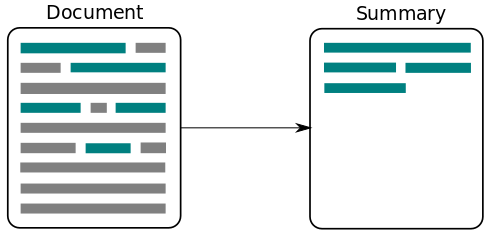
\includegraphics[width=0.6\linewidth]{./source/images/summarizationprocess.png}}
  \caption{Ablauf einer automatischen Zusammenfassung \cite{THA19}.}
  \label{pic:SummarizationProcess}
\end{figure}

\noindent
Mit besonderem Fokus auf das Gesundheitswesen lassen sich weiterhin zwei konkrete Einsatzgebiete konstruieren, in denen ein \ac{ATS}-Modell in einem ganzheitlichen System als autarkes Modul implementiert werden könnte. Einerseits ist die Zusammenfassung von Patientengesprächen denkbar, wenn eine entsprechende Spracherkennung mit integrierter Sprechererkennung vorgeschaltet ist. Die verdichteten Informationen ließen sich anschließend zum Beispiel in Patientenakten exportieren oder anderweitig klassifizieren. Andererseits können Pflegeroboter, welche mitunter demente Patienten betreuen, durch ein \ac{ATS}-Modell mit notwendigem Kontextwissen für die anstehenden Gespräche ausgestattet werden.
\newpage

\noindent
Die Anforderungen an ein \ac{ATS}-Modell lassen sich aus dem individuell anvisierten Einsatzgebiet ableiten und können anhand verschiedener Faktoren klassifiziert werden. Demnach kann man prinzipiell zwischen dem extraktiven und dem abstraktiven Ansatz differenzieren \cite[S.~5]{GAM16}. Extraktive Methoden bewerten die Sätze des ursprünglichen Textes anhand wort- und satzbezogener Attribute. Die Zusammenfassung entsteht sodann aus dem bewertungsgerechten Kopieren dieser Sätze \cite[S.~205-207]{KIA17}. Abstraktive Methoden hingegen verwenden Deep-Learning-Algorithmen, um Informationen zu identifizieren und entsprechende Zusammenfassungen mit völlig neuen Sätzen zu generieren \cite[S.~1]{NIT19}. Weiterhin ist zu entscheiden, ob einzelne oder mehrere Dokumente zusammengefasst werden sollen, welcher Domäne diese Dokumente entstammen und ob möglicherweise eine Dialogorientierung vorliegt.\\

\noindent
Aus technischer Sicht kommen bei der \ac{ATS} grundsätzlich Sequence-to-Sequence-Modelle zum Einsatz. Dabei wird stets eine Eingabesequenz $x = [x_{1}, ..., x_{n}]$ in eine Ausgabesequenz $y = [y_{1}, ..., y_{m}]$ überführt, wobei $n$ die Eingabelänge und $m$ die Ausgabelänge ist. Die Sequenzen werden von Vektoren repräsentiert. Mithin wird bei der \ac{ATS} $m$ \textless \, $n$ intendiert. Sequenzen bestehen hierbei aus Symbolen, also etwa Zeichen, Zeichenketten oder auch Ziffern. Architekturen modellieren also die bedingte Wahrscheinlichkeit $P(y \mid x)$ \cite[S.~32-33]{NIT19}. Die maßgebliche Herausforderung ist hierbei zum einen, dass \ac{ATS}-Modelle tatsächlich die wichtigsten Informationen einer Eingabesequenz identifizieren. Zum anderen gilt es, diese Informationen in eine entsprechende Ausgabesequenz zu integrieren. Eben diese Ausgabesequenz ist zudem orthographisch und grammatikalisch korrekt zu generieren. Üblicherweise wird dieser Vorgang auch als Paraphrasierung bezeichnet. Menschen müssen diese Fähigkeit ebenfalls erst einmal erlernen.


\section{Zielsetzung}
\noindent
Das Ziel dieser Arbeit ist dementsprechend die abstraktive Zusammenfassung einzelner Dokumente, wobei multilingual vortrainierte Modelle mittels \ac{TL} auf die deutsche Sprache adaptiert werden. Die Arbeit ist somit außerdem eine potenzielle Grundlage für die beiden konstruierten Einsatzgebiete aus dem Gesundheitswesen. Die Adaption auf die Domäne oder auch die Dialogorientierung ist nicht Teil dieser Arbeit.
\newpage

Die Forschungsfragen lauten wie folgt:

\begin{itemize}
	\item Wie lassen sich Texte automatisiert zusammenfassen?
	\item Wie können bereits existierende Modelle auf eine andere Sprache adaptiert werden?
	\item Wie qualitativ und skalierbar ist die Lösung?
\end{itemize}


\section{Aufbau der Arbeit}
\noindent
Nach der Einleitung werden zunächst die Grundlagen des \ac{DL} und des \ac{NLP} offengelegt. Im Kapitel des \ac{DL} werden neuronale Netze als solches definiert und ausgewählte Architekturen, welche auf die Zielerreichung einwirken, vorgestellt. Die Eigenschaften und die Relevanz von Hyperparametern und von \ac{TL} schließen sich an. Im Kapitel des \ac{NLP} werden neben der prinzipiellen Arbeit mit natürlicher Sprache und der entsprechenden Vorverarbeitung insbesondere sogenannte Word Embeddings und Deep Language Representations thematisiert.\\

\noindent
Bevor die bis dahin behandelten Komponenten in ein tatsächliches Modell integriert werden können, ist die Beschreibung der Datengrundlage erforderlich. Zum daran anschließenden abstraktiven Ansatz gehört die Erläuterung der Architektur, die Beschreibung des Trainingsprozesses und die Evaluation der Ergebnisse. Bei der sprachtechnischen Adaption des Modells auf die deutsche Sprache werden zuerst entsprechende Anpassungen an der ursprünglichen Architektur konzipiert, bevor erneut der Trainingsprozess beschrieben wird und die dazugehörigen Ergebnisse evaluiert werden. Der entsprechende Quellcode wird in Python entwickelt.


\section{Forschungsstand \& Referenzen}
\noindent
Aufgrund der stetig fortschreitenden Entwicklungen überholt sich der Forschungsstand der \ac{ATS} regelmäßig. Dennoch haben sich in den vergangenen Jahren gewisse Tendenzen erkennen lassen. Bereits zur Jahrtausendwende existierten erste \ac{ATS}-Systeme. Waren die ersten Ansätze zumeist noch extraktiv, wurde sich in den vergangenen Jahren mehr und mehr auf die abstraktiven Ansätze konzentriert. Vor 2016 schienen Ansätze mit \ac{RNN} und \ac{LSTM} sehr populär \cite{NAL16}. In den Jahren 2016 und 2017 etablierten sich Ansätze, welche auf \ac{RL} basierten \cite{PAU17}. Seit 2018 legten diverse Ansätze mit Encoder-Decoder-Architekturen die Grundlage des heutigen \ac{SOTA} \cite{YAN19, ROT20}, denn um den \ac{SOTA} konkurrieren fast ausschließlich sogenannte Transformer. Diese basieren auf den Encoder-Decoder-Architekturen, implementieren verschiedenartige Attention-Mechanismen und haben sich sowohl unter qualitativen als auch unter ökonomischen und ökologischen Aspekten bewiesen \cite{ZHA20}. Diese Arbeit wird daher ebenfalls diesen Ansatz verfolgen.\\

\noindent
Die Qualität der \ac{ATS} kann mithilfe des sogenannten ROUGE-Scores evaluiert werden. Dieser wird ebenso wie andere noch unerklärte Architekturen in einem nachfolgenden Kapitel dieser Arbeit umfangreich erläutert und kann zunächst als gegeben betrachtet werden. Die folgenden ROUGE-Scores können als zu reproduzierende Vergleichswerte verstanden werden: R-Recall: 15.96, R-Precision: 10.34, R-Measure: 12.22.\\

\noindent
Weiterhin hat der Durchbruch frei verfügbarer vortrainierter Modelle die \ac{NLP}-Welt revolutioniert, wie beispielsweise \ac{BERT} \cite{DEV19} oder auch \ac{ELMo} \cite{PET18} sowie deren Weiterentwicklungen. Verschiedenste \ac{NLP}-Aufgaben wie die \ac{ATS} konnten hiervon sehr stark profitieren. Die konkreten Funktionsweisen werden ebenfalls im Verlauf dieser Arbeit offengelegt. Wissenschaftliche Publikationen, welche mit dieser Arbeit vergleichbar sind und in dieser Arbeit oftmals referenziert werden, lauten wie folgt:

\begin{itemize}
	\item Text Summarization with Pre-Trained Encoders \cite{YAN19}
	\item German Abstractive Text Summarization using Deep Learning \cite{NIT19}
	\item Leveraging Pre-Trained Checkpoints for Sequence Generation \cite{ROT20}
\end{itemize}

\cleardoublepage

\chapter{Deep Learning}
\thispagestyle{fancy}
\label{chap:Deep Learning}

\noindent
Deep Learning ist ein Teilbereich des \ac{ML}. \ac{ML}-Algorithmen analysieren Daten automatisiert mittels mathematischer Methoden der Mustererkennung \cite[S.~455-457]{KHA19}. \ac{DL}-Algorithmen bedienen sich hingegen vielschichtiger und hoch parametrisierter neuronaler Netze, um dem menschlichen Gehirn bestmöglich nachzuempfinden und Anwendungen mit künstlicher Intelligenz auszustatten \cite[S.~1-2]{GOO16}. Dabei werden sehr große Datenmengen verarbeitet und analysiert, um einen Lerneffekt zu erzielen. Neben einer Eingabe- und einer Ausgabeschicht sorgen insbesondere die verborgenen Schichten für die beabsichtigte Tiefe. Hier werden Informationen weiterverarbeitet, abstrahiert und reduziert \cite[S.~164-165]{GOO16}. Der Aufbau neuronaler Netze sowie deren Funktionsweise und ausgewählte Architekturen werden in diesem Kapitel thematisiert. Hyperparameter und \ac{TL} schließen sich an.


\section{Neuronale Netze}
\noindent
Um den Aufbau und die Funktionsweise neuronaler Netze verstehen zu können, bedarf es zunächst der Beschreibung von Neuronen. Diese können im biologischen Sinne als Schalter verstanden werden, welche verschiedene Signale empfangen können und aktiviert werden, sobald ausreichend Signale registriert wurden. Diese Aktivierung sendet folglich weitere Signale an andere Neuronen, wie \autoref{pic:ArtificialNeuron} im technischen Sinne exemplarisch skizziert. Hierfür werden Aktivierungsfunktionen benötigt, welche die gewichteten Eingangssignale in ein Ausgangssignal konvertieren. Sie ermöglichen es, nicht-lineare Zusammenhänge zwischen den Eingangs- und den Ausgangsdaten herzustellen \cite[S.~134]{ZHA20}.
\newpage

\begin{figure}[h!]
  \centering
  \fbox{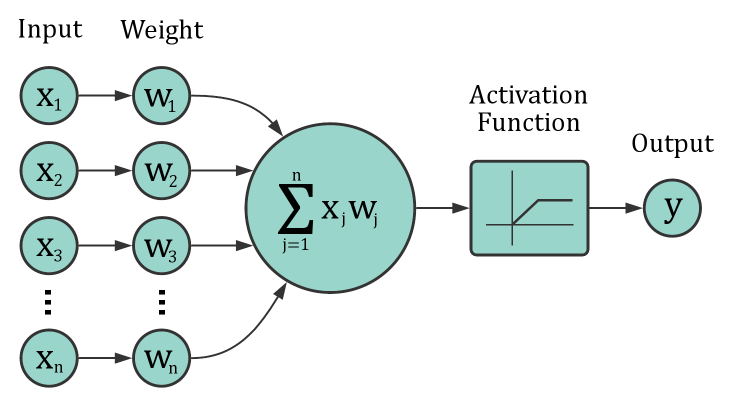
\includegraphics[width=0.6\linewidth]{./source/images/artificialneuron.png}}
  \caption{Aufbau eines künstlichen Neurons \cite{MCC20}.}
  \label{pic:ArtificialNeuron}
\end{figure}

\noindent
Die elementarste Form neuronaler Netze wird \ac{MLP} genannt. \ac{MLP} bestehen aus mehreren Schichten, deren Neuronen jeweils vollständig mit den Neuronen der umliegenden Schichten verbunden sind \cite[S.~131]{ZHA20}. Der Verständlichkeit halber veranschaulicht \autoref{pic:MultiLayerPerceptron} einen solchen Aufbau mit nur einer verborgenen Schicht (engl. Hidden Layer), welche aus fünf Neuronen besteht. Dabei zeichnen sich vollvermaschte Schichten (engl. Fully Connected Layer oder Dense Layer) dadurch aus, dass alle Neuronen mit allen Inputs und Outputs verbunden sind.\\

\begin{figure}[h!]
  \centering
  \fbox{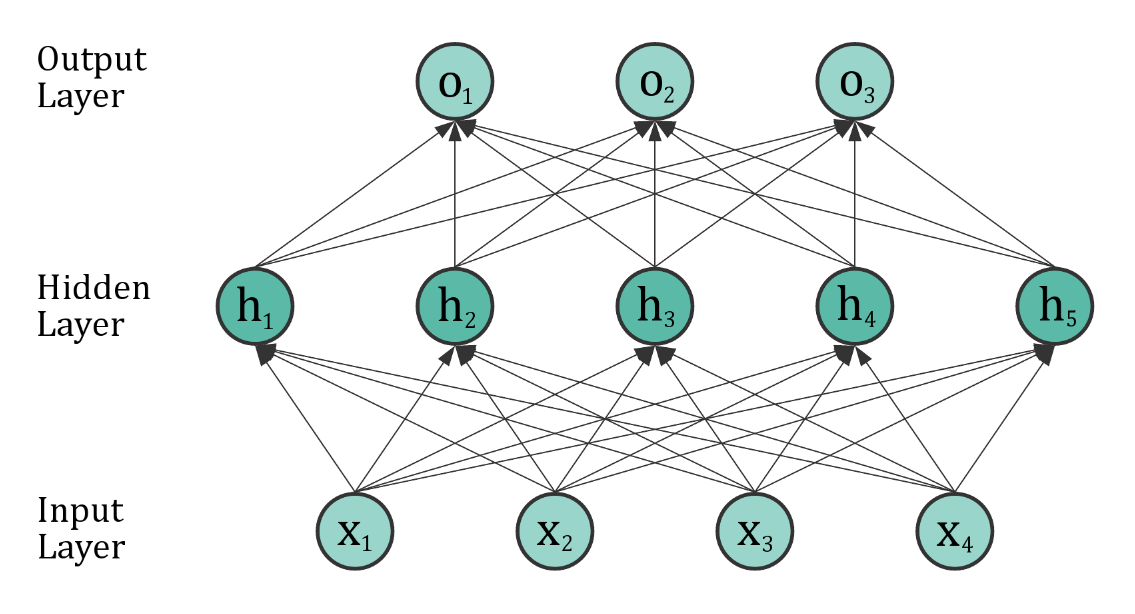
\includegraphics[width=0.65\linewidth]{./source/images/multilayerperceptron.png}}
  \caption{Aufbau eines MLP \cite[S.~388]{RAS19}.}
  \label{pic:MultiLayerPerceptron}
\end{figure}

\noindent
Ziel der hoch parametrisierten neuronalen Netze ist es, komplexe Polynomfunktionen höheren Grades bestmöglich zu approximieren und so verschiedenste Probleme zu lösen. Der Grad einer Polynomfunktion wird an der höchsten Potenz des jeweiligen Funktionsterms gemessen.
\newpage

\noindent
Der anvisierte Lerneffekt wird mithilfe des sogenannten Backpropagation-Algorithmus erreicht. Hierbei werden Eingangsdaten zunächst vorwärts durch ein neuronales Netz hindurch propagiert. Mithilfe einer Fehlerfunktion wird sodann die erwartete mit der tatsächlichen Ausgabe verglichen und bewertet. Demzufolge sind gelabelte Daten erforderlich, um das hier beschriebene überwachte Training (engl. Supervised Learning) ausführen zu können \cite[S.~3]{RAS19}. Über das Gradientenverfahren werden die Fehler nun rückwärts durch das neuronale Netz propagiert und somit die Gewichte in den Neuronen angepasst, insbesondere in den verborgenen Schichten. Ziel ist die Minimierung der Fehlerfunktion und letztlich die Optimierung der durch das neuronale Netz approximierten Funktion. \autoref{pic:SupervisedLearning} verdeutlicht nochmals die Funktionsweise von überwachten Lernalgorithmen, welche in Folge eines Trainingsprozesses unbekannte Daten verarbeiten können \cite[S.~167-169]{ZHA20}.\\

\begin{figure}[h!]
  \centering
  \fbox{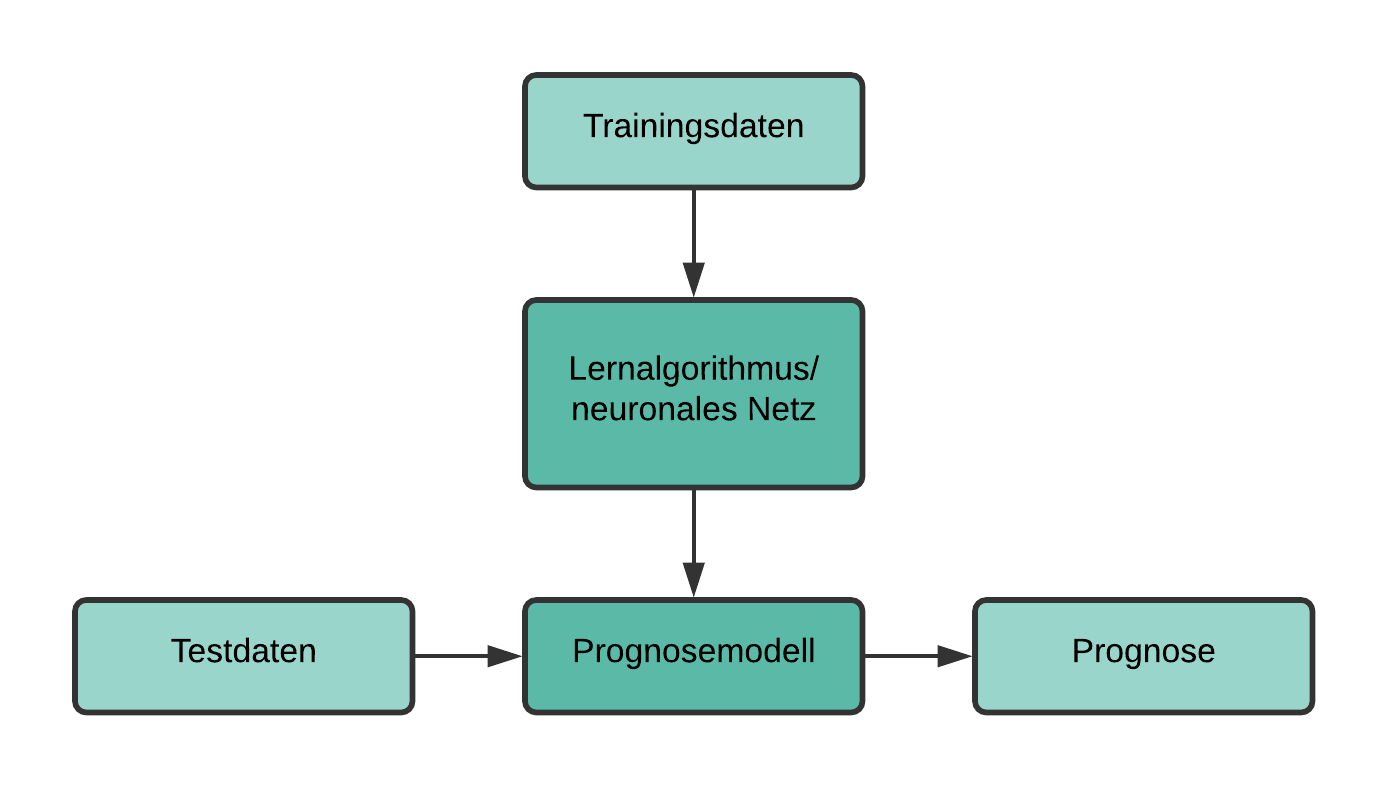
\includegraphics[width=0.7\linewidth]{./source/images/supervisedlearning.png}}
  \caption{Supervised Learning \cite[S.~3]{RAS19}.}
  \label{pic:SupervisedLearning}
\end{figure}

\noindent
Der Trainingsprozess erfolgt über mehrere sogenannte Epochen. Hier werden dem neuronalen Netz die Eingangsdaten zugeführt und beidseitige Propagationen ausgeführt. Hierbei ist wichtig, kein Over- oder Underfitting zu erzeugen. Dies würde bedeuten, dass das trainierte Modell zu sehr oder zu wenig auf die Trainingsdaten angepasst ist. Ziel ist ein möglichst hoher Generalisierungseffekt des Modells, wie \autoref{pic:FittingTypes} zeigt. Das Modell sollte den Lernfortschritt auf unbekannte Daten adaptieren können und darauf eine hohe Genauigkeit erreichen \cite[S.~108-110]{GOO16}. Es gibt verschiedene Ansätze, um beispielsweise Overfitting vorzubeugen. Hier seien Batch Normalization, Dropout und Early Stopping genannt, wobei entsprechende Mechanismen an anderweitiger Stelle erläutert werden \cite[S.~241,~255,~276,~313]{GOO16}.\\

\begin{figure}[h!]
  \centering
  \fbox{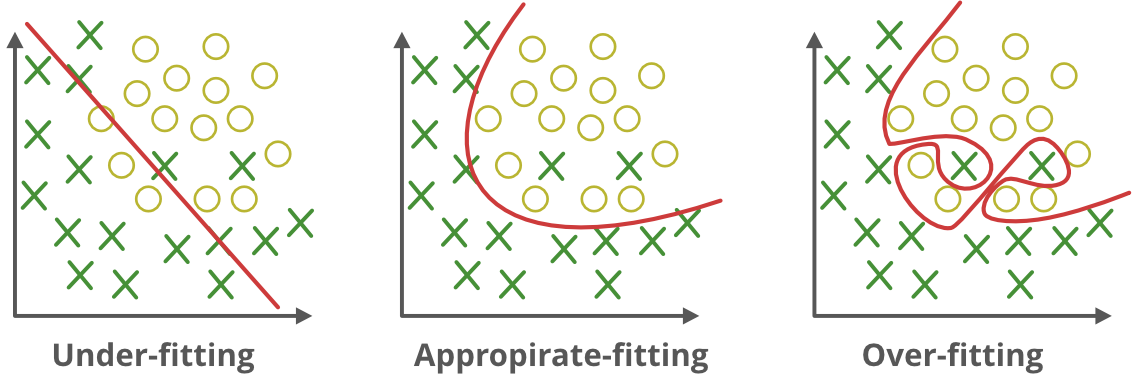
\includegraphics[width=0.75\linewidth]{./source/images/fittingtypes.png}}
  \caption{Typen von Generalisierungseffekten \cite{EDPOJ}.}
  \label{pic:FittingTypes}
\end{figure}


\section{Architekturen}
\noindent
Um die \ac{ATS} mithilfe neuronaler Netze zu modellieren, werden nun ausgewählte Architekturen vorgestellt. Diese gehen weit über die als Grundlage beschriebenen \ac{MLP} hinaus. Eingangsdaten der \ac{ATS} haben in jedem Fall einen Textcharakter. Dabei ist die Reihenfolge der Sätze und der Wörter von großer Bedeutung, um Texte hinreichend verstehen und anschließend generieren zu können. Dies wird von den nachfolgend beschriebenen Architekturen gewährleistet \cite[S.~301]{ZHA20}.


\subsection{Encoder-Decoder-Networks}
\noindent
Encoder-Decoder-Architekturen sind zunächst einmal als Template zu verstehen, welches einer stets individuellen Entwicklung bedarf. Dabei bestehen entsprechende Modelle aus einem Encoder und einem Decoder. Beide Module bestehen aus neuronalen Netzen, welche beispielsweise durch \ac{RNN} oder auch \ac{LSTM} repräsentiert werden können. Hierdurch würde zugleich die Verarbeitung sequenzieller Daten ermöglicht. Hinsichtlich der anvisierten \ac{ATS} spricht man daher auch von Sequence-to-Sequence-Modellen \cite[S.~2]{VAS17}.\\

\noindent
Im Encoder wird die Eingabesequenz zuerst eingebettet. Dabei entsteht ein Merkmalsvektor, welcher entlang eines zugrundeliegenden Wortschatzes aus den Indizes der eingegangenen Wörter besteht. Er ist die mathematisch verarbeitbare Version der Eingabesequenz. Dieser Vorgang wird im weiteren Verlauf dieser Arbeit noch hinreichend beschrieben und untersucht. Der Merkmalsvektor geht sodann in das neuronale Netz des Encoders ein und wird in eine entsprechende Zustandsrepräsentation überführt.
\newpage

\noindent
Der Decoder wird mit eben diesen Ausgangsdaten des Encoders initialisiert. Die entsprechende Zustandsrepräsentation wird ebenfalls mithilfe eines neuronalen Netzes verarbeitet \cite[S.~2]{VAS17}. Nun wird jedoch zusätzlich eine Ausgabesequenz generiert, welche der \ac{ATS} gerecht werden soll. Wie bereits bekannt ist, gilt es letztlich die bedingte Wahrscheinlichkeit $P(y \mid x)$ zu modellieren \cite{YAN19}.\\

\noindent
Es folgt nun eine mathematische Betrachtung der Encoder-Decoder-Architektur. Hierfür wird die genannte Zustandsrepräsentation als Kontextvektor $c$ bezeichnet. Die Wahrscheinlichkeit für eine Ausgabe am Index $t > 0$ kann demnach mit $$P(y_t \mid y_1, ..., y_{t-1}, c)$$ modelliert werden. Die Berechnung der verborgenen Zustände im Decoder erfordert nun den Merkmalsvektor, den Kontextvektor und den letzten verborgenen Zustand des Encoders. Hiermit kann $$h_t = f(y_{t-1}, c, h_{t-1})$$ berechnet werden. Informationen, welche an vorherigen Indizes gespeichert sind, können rekursiv ermittelt werden. Architektonisch ist weiterhin zu beachten, dass die Konfiguration des Encoders der Konfiguration des Decoders gleicht \cite[S.~2]{VAS17}.\\

\noindent
Um die theoretisch und abstrakt beschriebene Architektur zu veranschaulichen, werden die wesentlichen Module nun abschließend in \autoref{pic:EncoderDecoder} visuell in Zusammenhang gebracht. Allgemein gilt: Eine Eingabesequenz $x = [x_{1}, ..., x_{n}]$ wird mithilfe des Encoders zunächst in einen kontinuierlichen Zustandsvektor $z = [z_{1}, ..., z_{n}]$ überführt, bevor der Decoder daraus die Ausgabesequenz $y = [y_{1}, ..., y_{m}]$ generieren kann \cite[S.~2]{VAS17}.\\

\begin{figure}[h!]
  \centering
  \fbox{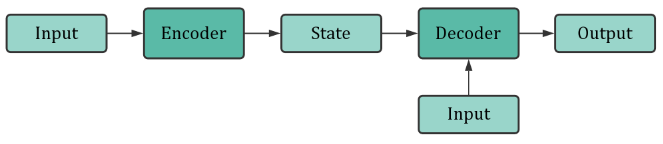
\includegraphics[width=0.75\linewidth]{./source/images/encoderdecoder.png}}
  \caption{Encoder-Decoder-Architektur \cite[S.~375]{ZHA20}.}
  \label{pic:EncoderDecoder}
\end{figure}
\newpage


\subsection{Attention in Neural Networks}
\noindent
Die Encoder-Decoder-Architektur kann im Kontext der \ac{ATS} um einen sogenannten Attention-Mechanismus erweitert werden, welcher den Encoder mit dem Decoder verbindet. Dabei geht es der Übersetzung folgend um Aufmerksamkeit. In der kognitiven Neurowissenschaft wird Aufmerksamkeit als ein Zustand gesteigerter Anspannung definiert, welcher selektive Wahrnehmung sowie entsprechendes Denken und Handeln umfasst. Diese Fähigkeit wird von einem \ac{ATS}-Modell verlangt und mithilfe der nachfolgend beschriebenen \ac{SDPA} realisiert. Um letztlich eine qualitative Zusammenfassung generieren zu können, selektiert der Attention-Mechanismus die wichtigsten Informationen aus dem Encoder, indem er die dort verarbeitete Eingabesequenz stets beobachtet und globale Zusammenhänge zwischen der Eingabesequenz und der Ausgabesequenz herstellt. Der Decoder wird dementsprechend darüber informiert \cite[S.~1]{VAS17}. Das \ac{ATS}-Modell soll mathematisch also menschenähnlichem Verhalten nachempfinden \cite[S.~389]{ZHA20}.\\

\noindent
Die \ac{SDPA} besteht hierfür aus einer Attention-Funktion, welche Queries und eine Menge von Key-Value-Paaren verarbeiten kann. Hierbei gehen Queries und Keys der Dimension $d_k$ sowie Values der Dimension $d_v$ ein. Die \ac{SDPA} kann somit gemäß $$Attention(Q, K, V) = Softmax(\frac{Q \cdot K^T}{\sqrt{d_k}}) \cdot V$$ berechnet werden, indem das Skalarprodukt der Queries und Keys berechnet, durch einen dimensionsabhängigen Term dividiert und unter Anwendung einer Softmax-Funktion mit den Values multipliziert wird \cite[S.~4]{VAS17}.\\

\noindent
Die \ac{SDPA} kann innerhalb einer Encoder-Decoder-Architektur wie folgt an einem Index $t$ integriert werden. Der Encoder bettet die Eingabesequenz in bekannter Weise ein und verarbeitet sie, indem die verborgenen Zustände über alle verborgenen Schichten hinweg berechnet werden. Die Attention-Schicht erhält in der Folge alle Informationen, die der Encoder verarbeitet hat. Der Decoder wird nicht nur über den vorangegangenen verborgenen Zustand des Encoders informiert, sondern auch über den aus der Attention-Schicht resultierenden Kontext. Dieser wird als Antwort auf eine Query generiert, wobei diese Query wiederum durch den vorangegangenen verborgenen Zustand des Decoders repräsentiert wird. Die Ausgabesequenz wird hierbei indexweise und autoregressiv generiert, da dem Decoder in jedem Index zusätzlich die bereits generierten Wörter zugeführt werden \cite[S.~5]{VAS17}.
\newpage

\noindent
Weiterhin wird zwischen zwei Eigenarten unterschieden: Self-Attention und Multi-Head-Attention. Self-Attention transformiert innerhalb einer Query $n$ Inputs in $n$ Outputs. Dabei interagieren alle Inputs miteinander, um die Verteilung der globalen Attention zu bestimmen. Die Outputs entstehen folglich, indem die entsprechenden Scores aggregiert werden. Betrachtet man also einen Satz, dann ist die Attention jedes darin enthaltenen Wortes zu berechnen \cite{KAR19}. \autoref{pic:SelfAttention} visualisiert diese Self-Attention.\\

\begin{figure}[h!]
  \centering
  \fbox{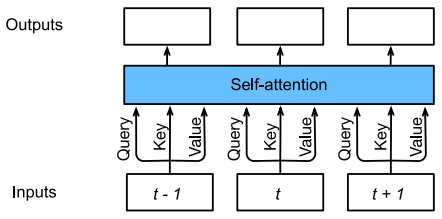
\includegraphics[width=0.5\linewidth]{./source/images/selfattention.png}}
  \caption{Self-Attention \cite[S.~400]{ZHA20}.}
  \label{pic:SelfAttention}
\end{figure}

\noindent
Multi-Head-Attention hingegen betrachtet direkt mehrere Queries. Die Matrizen der Queries Q, Keys K und Values V werden mithilfe entsprechender Gewichtsmatrizen dimensional reduziert, um $$Head = Attention(QW^Q, KW^K, VW^V)$$ zu berechnen. Diese Berechnung geschieht h-mal, sodass entsprechend viele Heads in Form von Gewichtsmatrizen entstehen. Diese werden konkateniert und wiederum mit entsprechenden Gewichtsmatrizen transformiert, sodass $$MultiHead(Q,K,V) = Concat(Head_1, ..., Head_h) \cdot W^O$$

\noindent
gilt. Hierdurch wird es dem Modell ermöglicht, Informationen aus verschiedenen Repräsentationen zu identifizieren. Betrachtet man also erneut einen Satz, dann werden die Informationen positionsunabhängig und satzübergreifend identifiziert \cite{VAS17}. \autoref{pic:MultiHeadAttention} visualisiert die Multi-Head-Attention architektonisch.
\newpage

\begin{figure}[h!]
  \centering
  \fbox{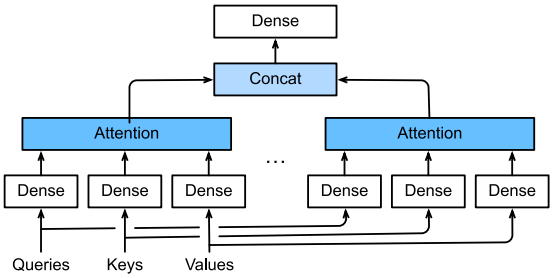
\includegraphics[width=0.75\linewidth]{./source/images/multiheadattention.png}}
  \caption{Multi-Head-Attention \cite[S.~400]{ZHA20}.}
  \label{pic:MultiHeadAttention}
\end{figure}


\subsection{Transformer Networks}
\noindent
Transformer basieren ebenfalls auf der Encoder-Decoder-Architektur, wobei darüber hinaus verschiedene Attention-Mechanismen implementiert werden. Besonders ist hierbei, dass die Eingabesequenz parallel zur Anwendung der Attention-Mechanismen positionsabhängig eingebettet wird, um sequenzielle Informationen zu extrahieren. Dies führt insgesamt zu einem recht kompatiblen Modell, welches nur noch einer stark verringerten Trainingszeit bedarf \cite[S.~5-6]{VAS17}.\\

\noindent
Architektonisch werden die Schichten bisheriger Sequence-to-Sequence-Modelle durch Transformer-Module ersetzt. Diese bestehen aus einer Multi-Head-Attention-Schicht, einem positionsabhängigen Feed-Forward-Netzwerk und einer Layer-Normalization-Schicht. Eben diese wird benötigt, um für das entsprechende Modell einen generalisierenden Effekt zu erzielen. Transformer-Module analysieren die eingehenden Wörter unabhängig voneinander. Daher ist es wichtig, die Eingabesequenz positionsabhängig einzubetten, wie oben bereits angedeutet wurde. Hierdurch können sequenzielle Informationen extrahiert werden. Dabei werden überdies keine neuen Abhängigkeiten erlernt, wohl aber die Trainingszeit weiter reduziert \cite[S.~399-404]{ZHA20}. \autoref{pic:TransformerArchitecture} visualisiert die beschriebene Architektur.
\newpage

\begin{figure}[h!]
  \centering
  \fbox{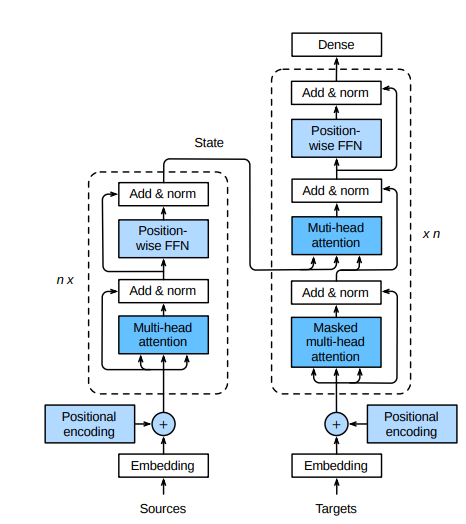
\includegraphics[width=0.7\linewidth]{./source/images/transformerarchitecture.png}}
  \caption{Transformer-Architektur \cite[S.~3]{VAS17}.}
  \label{pic:TransformerArchitecture}
\end{figure}

\noindent
Zuletzt ist wichtig, dass Transformer und ihre Komponenten verschiedenartig konzipiert werden können. Dies wird stets durch das anvisierte Ziel bedingt. Eine hinsichtlich der \ac{ATS} geeignete Architektur wird in einem entsprechenden Kapitel noch umfangreicher offengelegt. Zudem können bestimmte Komponenten der Transformer durch vortrainierte Modelle repräsentiert werden. Dies wird ebenfalls im weiteren Verlauf dieser Arbeit thematisiert, nachdem entsprechende Grundlagen dargelegt wurden.
\newpage


\section{Hyperparameter}
\noindent
Hyperparameter sind Parameter einer Architektur, die bereits vor dem eigentlichen Trainingsprozess definiert werden. Sie bedürfen einer separaten Optimierung, da sie eben dieses Training und folglich auch die Qualität des entstehenden Modells enorm beeinflussen. Ziel ist es hierbei, die beste Kombination aller Hyperparameter zu finden, um die Fehlerfunktion hinreichend zu minimieren \cite[S.~1]{YAN20}.\\

\noindent
Dies wird im Trainingsprozess als Teil der Backpropagation durch das Gradientenverfahren erreicht, welches die methodische Lösung allgemeiner Optimierungsprobleme übernimmt. Entlang eines negativen Gradienten wird das globale Minimum der dazugehörigen Fehlerfunktion gesucht, bis keine numerische Verbesserung mehr zu verzeichnen ist \cite[S.~428]{ZHA20}. Im weiteren Verlauf werden ausgewählte Hyperparameter, welche das Gradientenverfahren und damit den allgemeinen Trainingsprozess hochgradig beeinflussen, vorgestellt.\\

\noindent
Die \ac{LR} ist ein Hyperparameter, der bestimmt, wie viel Einfluss jede einzelne Epoche im Trainingsprozess auf die Anpassung der Gewichte nimmt. Sie gilt mithin als wichtigster Hyperparameter einer Architektur \cite[S.~208]{GOO16}. Eine zu niedrige \ac{LR} kann den Trainingsprozess entweder stark verlangsamen oder dafür sorgen, dass kein Lernfortschritt mehr erzielt wird, da lokale Minima der Fehlerfunktion nicht übersprungen werden können und fälschlicherweise als globales Minimum interpretiert werden. Eine zu hohe \ac{LR} kann hingegen sehr abrupte Anpassungen der Gewichte verursachen, sodass potenziell auch das globale Minimum übersprungen werden kann \cite[S.~414-415]{ZHA20}. \autoref{pic:GradientDescent} verdeutlicht diese Bedingungen. Ziel ist allgemein eine möglichst schnelle Konvergenz.\\

\begin{figure}[h!]
  \centering
  \fbox{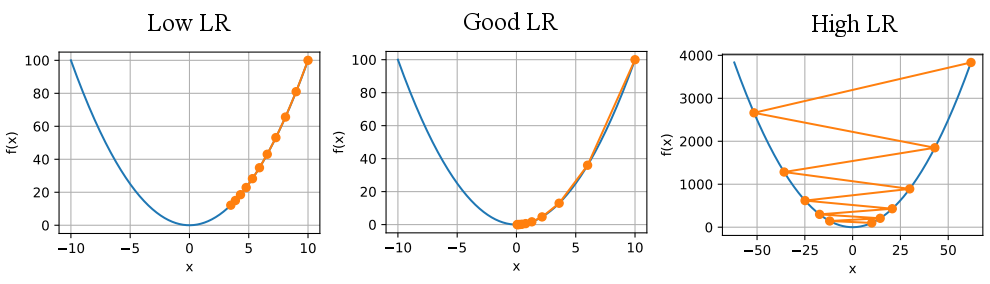
\includegraphics[width=0.7\linewidth]{./source/images/gradientdescent.png}}
  \caption{Konvergenzverhalten im Gradientenverfahren \cite[S.~429]{ZHA20}.}
  \label{pic:GradientDescent}
\end{figure}
\newpage

\noindent
Neben der sorgfältigen manuellen Auswahl der \ac{LR}, etwa mithilfe eines sogenannten \ac{LR}-Schedule, ist es weiterhin möglich, eine adaptive \ac{LR} einzuführen. Hierbei wird die \ac{LR} in jeder Epoche verändert. Üblich ist hier eine Reduktion der \ac{LR}, wenn bereits akzeptable Ergebnisse erreicht wurden \cite[S.~433]{ZHA20}.\\

\noindent
Außerdem existiert das stochastische Gradientenverfahren, welches pro Epoche nur eine Stichprobe der verfügbaren Trainingsdaten berücksichtigt und einen generalisierenden Effekt verspricht \cite[S.~290]{GOO16}. Die Größe der Stichprobe wird üblicherweise als Batch Size bezeichnet und an dieser Stelle nur als weitergehender Hyperparameter genannt.\\

\noindent
Weiterhin unterstützt das Momentum die bereits beschriebene \ac{LR} auf der Suche nach dem globalen Minimum in der Fehlerfunktion. Dabei berücksichtigt es den Durchschnitt vorheriger Gradienten. Auf dieser Grundlage wird entschieden, in welche Richtung das stochastische Gradientenverfahren weiter absteigen soll, wie \autoref{pic:MomentumUpdate} zeigt. Das Momentum ist somit potenziell in der Lage, lokale Minima zu überspringen und die Suche erst im tatsächlichen globalen Minimum zu beenden \cite[S.~292-295]{GOO16}.\\

\begin{figure}[h!]
  \centering
  \fbox{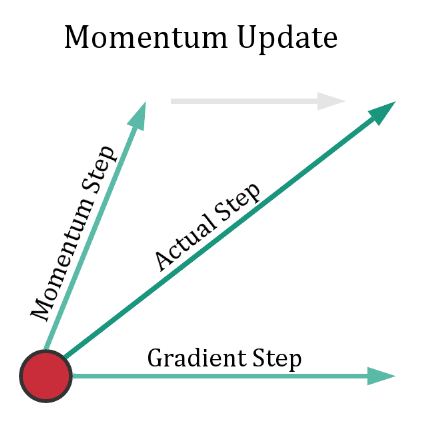
\includegraphics[width=0.3\linewidth]{./source/images/momentumupdate.png}}
  \caption{Gradientenverfahren unter Einfluss eines Momentums \cite{CSNOJ}.}
  \label{pic:MomentumUpdate}
\end{figure}

\noindent
Bei der Auswahl eines hohen Momentums sollte die \ac{LR} eher niedriger sein, oder anders herum. Eine Möglichkeit der stochastischen Optimierung ist hierbei \ac{ADAM}. Dieser Algorithmus übernimmt nicht nur die Auswahl der adaptiven \ac{LR}, sondern auch die Auswahl des entsprechenden Momentums. \ac{ADAM} arbeitet weitreichenden Analysen zufolge effizient für daten- und parameterintensive Probleme. Dabei konvergiert der Algorithmus üblicherweise schneller als vergleichbare Optimierungsalgorithmen \cite[S.~1-2]{KIN17}.\\

\noindent
Zuletzt ist noch das Weight Decay erwähnenswert. Dieses meint die Multiplikation der Gewichte einer Architektur nach jeder Epoche mit einem Faktor kleiner als eins, um sehr große Gewichte zu verhindern. Die Gefahr von Overfitting wird hierbei verringert, während sich die Generalisierung des Modells verbessert. Allgemein lässt sich die optimale Kombination aller Hyperparameter auch durch Techniken wie Grid Search (vgl. Brute-Force) annähern \cite[S.~24]{YAN20}.


\section{Transfer Learning}
\noindent
\ac{TL} ist in den letzten Jahren wissenschaftlich immer bedeutsamer geworden, da \ac{DL}-Modelle heutzutage sehr komplex und Trainingsprozesse sehr zeit- und rechenintensiv sind. Unter \ac{TL} versteht man das Wiederverwenden bereits vortrainierter neuronaler Netze für die Lösung neuartiger Probleme. Das initiale Training obliegt hierbei meist großen Unternehmen oder Institutionen. Dabei werden die erprobten Modelle sodann als Startpunkt genutzt und nur noch auf die neuen Probleme adaptiert, anstatt eigene Modelle von Grund auf neu zu trainieren. Anwender profitieren hier zeitlich, qualitativ und technisch. Zumeist sind architektonische Anpassungen in den hinteren Schichten der vortrainierten Modelle erforderlich, sodass sie sich für die Lösung der neuen Probleme eignen, wie \autoref{pic:FineTuning} veranschaulicht. Zudem ist ein gezieltes weitergehendes Training (engl. Fine-Tuning) mit entsprechenden Daten notwendig. Inwieweit die neuen Daten auf die vortrainierten Modelle einwirken sollen, ist individuell zu erproben \cite[S.~319,~534]{GOO16}.\\

\begin{figure}[h]
  \centering
  \fbox{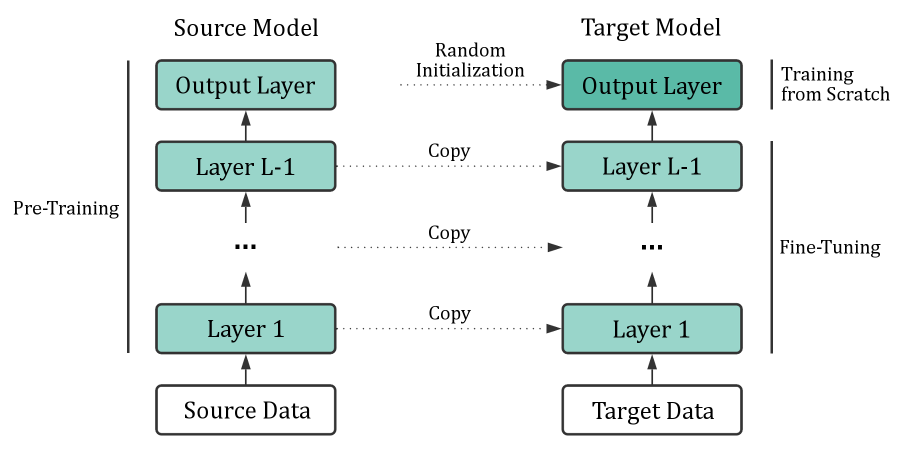
\includegraphics[width=0.7\linewidth]{./source/images/finetuning.png}}
  \caption{Fine-Tuning vortrainierter Modelle \cite[S.~555]{ZHA20}.}
  \label{pic:FineTuning}
\end{figure}
\newpage

\noindent
\ac{TL} wird auch in dieser Arbeit genutzt. Einige Komponenten der bereits vorgestellten Architekturen, wie beispielsweise der Encoder oder auch der Decoder, können durch vortrainierte Modelle repräsentiert werden. Hier wird inhaltlich sowie kontextuell in den folgenden Kapiteln angeknüpft, da zunächst die Einführung weiterer \ac{NLP}-Grundlagen erforderlich ist. Die angeführten Vorteile von \ac{TL} können nichtsdestotrotz folgendermaßen zusammengefasst werden:

\begin{itemize}
	\item Zeitersparnis durch Überspringen des initialen Trainings
	\item Qualitätsanstieg und Generalisierung durch Zuführung massenhafter Daten
	\item Reduktion von Anforderungen, Kosten und Stromverbrauch beim Fine-Tuning
\end{itemize}

\cleardoublepage

\chapter{Natural Language Processing}
\thispagestyle{fancy}
\label{chap:Natural Language Processing}

\noindent
Natürliche Sprache wird auch als menschliche Sprache bezeichnet und ist historisch gewachsen. Sie verfolgt orthographische und grammatikalische Regeln auf Grundlage eines sprachabhängigen Wortschatzes. Die Sprachwissenschaft, auch Linguistik genannt, untersucht natürliche Sprache mithilfe verschiedener Methoden. \ac{NLP} meint die maschinelle Verarbeitung natürlicher Sprache. Dabei werden Methoden der Linguistik unter anderem mit Methoden des Deep Learning verknüpft \cite[S.~1]{BIR09}. Nicht selten ist eine Spracherkennung vorgeschaltet. \ac{NLP} ist weiterhin in \ac{NLU} und \ac{NLG} zu untergliedern \cite[S.~27-28]{BIR09}. Diese Teilgebiete sind zugleich wesentliche Herausforderungen der \ac{ATS}.\\

\noindent
\ac{NLP}-Aufgaben sind oftmals als Optimierungsprobleme zu verstehen. Lösungen sind demnach nicht eindeutig, also im mathematischen Sinne analytisch nicht lösbar. Dies wird in Hinblick auf die \ac{ATS} deutlich, wenn man verschiedene Personen den gleichen Text zusammenfassen lässt. Zwar gleichen sich die als relevant identifizierten Informationen größtenteils, doch die Formulierungen sind mitunter sehr unterschiedlich. Folglich können auch mehrere Versionen korrekt sein.\\

\noindent
Natürliche Sprache bedarf hinsichtlich maschineller Verarbeitung einer geeigneten mathematischen Form. Hierfür werden nachfolgend verschiedene Vorverarbeitungsschritte sowie Word Embeddings und Deep Language Representations vorgestellt. Der Anspruch auf Vollständigkeit entfällt aufgrund der Mächtigkeit des \ac{NLP}, obgleich anknüpfende Inhalte bei Bedarf an den entsprechenden Stellen erläutert werden.
\newpage


\section{Vorverarbeitung}
\noindent
In nahezu allen Teilbereichen der Data Science stehen gewöhnlicherweise etliche Vorverarbeitungsschritte an, um die zu analysierenden Daten zu bereinigen, zu normalisieren und insgesamt in eine konsistente sowie geeignete Form zu bringen. Im \ac{NLP}-Kontext sind indes komplexere Vorverarbeitungsschritte erforderlich, um die Daten für die eingeforderte mathematische Form zu präparieren \cite[S.~86]{BIR09}. Eine Auswahl der in dieser Arbeit relevanten Schritte wird nachfolgend vorgestellt. In der Implementierung dieser chronologisch aufeinander folgenden Schritte spricht man auch von der \ac{NLP}-Pipeline.


\subsection{Textbereinigung}
\noindent
An erster Stelle der \ac{NLP}-Pipeline steht die Textbereinigung, welche sich bezüglich eingehender Sequenzen insbesondere auf Sonderzeichen, Interpunktion sowie Klein- und Großschreibung konzentriert. Dabei ist es mitunter bereits herausfordernd, entsprechende Textstellen als solche zu identifizieren. Anschließend sind oftmals normalisierende Maßnahmen anzuwenden. Üblich ist beispielsweise das Entfernen von Sonderzeichen oder auch das Erzwingen von Kleinschreibung in allen eingehenden Texten \cite[S.~107]{BIR09}. Weit verbreitet ist auch das Entfernen von Stoppwörtern. Dies sind Wörter, welche mutmaßlich der Allgemeinsprache zugehören, weshalb angenommen wird, dass sie keine entscheidende inhaltliche Bedeutung besitzen \cite[S.~5]{GAM16}. Hier lässt sich jedoch keine allgemeingültige Aussage treffen, da die tatsächlich erforderlichen Maßnahmen sowohl von den Eigenschaften der Eingangsdaten als auch von den Besonderheiten der verwendeten Modelle und den verfolgten Zielen abhängen. Dabei ist die Datenexploration wiederkehrend und alternierend mit der Anpassung der Vorverarbeitung auszuführen. Der Anwender sollte hierbei ein Gefühl für die Daten und deren Besonderheiten entwickeln. Zudem bedarf es einem tiefgründigen Verständnis der geplanten Aufgaben, um beurteilen zu können, welche Vorverarbeitungsschritte tatsächlich relevant sind.


\subsection{Textnormalisierung}
\noindent
In der weitergehenden Textnormalisierung wird sich vorrangig auf das Stemming und die Lemmatisierung konzentriert. Das Stemming führt eingehende Wörter auf ihre Grundformen zurück, indem bekannte Präfixe, Infixe und Suffixe eliminiert werden. Diese Grundformen sind nicht zwingend valide Wörter. Die Lemmatisierung hingegen berücksichtigt die wortspezifischen Bedeutungen, um etwaige Flexionen in Deckung zu bringen und somit die linguistisch korrekten Grundformen zu bilden. Flexionen sind durch Konjugationen, Deklinationen oder auch Komparationen entstanden und natürlicher Bestandteil einer Sprache. Hierfür sind Wortbildungsregeln und ein Wortschatz erforderlich. Letzterer indiziert die eingehenden Wörter anhand ihrer Lemmata und ordnet sie entsprechend zu \cite[S.~107-108]{BIR09}. Zwar ist die Lemmatisierung aufgrund des erforderlichen Kontextwissens durchaus komplexer als das Stemming, dafür sind ihre Ergebnisse erwartungsgemäß gehaltvoller. Ob und welche Methode zur Textnormalisierung herangezogen wird, hängt erneut von der anvisierten Aufgabe ab. Seien nun beispielhaft die Wörter \{\textit{spielen, spielst, spielte, gespielt}\} gegeben, dann reduziert der Stemmer diese Wörter auf die Grundform \textit{spiel}. Der Lemmatizer identifiziert hingegen die linguistisch korrekte Grundform \textit{spielen}.\\

\noindent
\ac{NLTK} ist eine forschungsorientierte Python-Bibliothek, die etliche \ac{NLP}-Module zur Verfügung stellt, darunter unter anderem verschiedenartige Stemmer \cite[S.~13-14]{BIR09}. Stemmer, welche die englische Sprache unterstützen, scheinen bereits sehr ausgereift zu sein. Stemmer, welche die deutsche Sprache unterstützen, sind nicht nur knapp, sondern bedürfen zudem weitergehenden Testschritten, um deren tatsächliche Eignung zu prüfen. Die Stemmer nltk.stem.cistem und nltk.stem.snowball eignen sich potenziell für einen Einsatz mit deutscher Sprache \cite{NLT20}.\\

\noindent
SpaCy ist eine eher praktisch orientierte Python-Bibliothek für verschiedenste \ac{NLP}-Aufgaben. Hinsichtlich der deutschen Sprache eignen sich hier insbesondere die verfügbaren Lemmatizer. Dabei kann der Anwender zwischen verschiedenen vortrainierten Modellen wählen. Eigenschaften wie Sprache, Größe und zugrundeliegende Trainingsdaten sind transparent dokumentiert \cite{SPA21}.\\

\noindent
Die Wahl geeigneter Stemmer und Lemmatizer obliegt dennoch den subjektiven Präferenzen des jeweiligen Entwicklers. In jedem Fall sind hinreichende Tests durchzuführen, um die einzelnen Module zu erproben sowie individuelle Vor- und Nachteile zu identifizieren. Mit fortschreitender Entwicklung beweisen sich möglicherweise auch andere aufstrebende Bibliotheken \cite[S.~108]{BIR09}.
\newpage


\subsection{Tokenisierung}
\noindent
In der Tokenisierung werden Texte in logisch zusammengehörige Token zerlegt. Texte bestehen aus Sequenzen, welche wiederum aus Symbolen, also etwa Zeichen, Zeichenketten oder auch Ziffern bestehen. Token sind indes als Einheiten der Wort- oder Satzebene zu verstehen \cite[S.~22-24]{MAN08}.\\

\noindent
Der einfachste Ansatz einer wortbasierten Tokenisierung besteht darin, den Text anhand von Leerzeichen und nicht-alphanumerischer Zeichen zu segmentieren. Dies ist jedoch nicht völlig obligatorisch und führt meist nicht zu einer verarbeitbaren Lösung, weshalb sprachabhängige Eigenarten berücksichtigt werden müssen. Typisch ist beispielsweise die Weiterbehandlung von vor- oder nachstehenden Klammern an den Token \cite[S.~109-111]{BIR09}.\\

\noindent
Ob weiterhin auch Interpunktion berücksichtigt oder verworfen werden soll, ist hinsichtlich der anvisierten \ac{NLP}-Aufgabe individuell zu entscheiden und zu erproben. Gleiches gilt für die Entscheidung, ob eingehende Texte roh oder vorverarbeitet hineingegeben werden.\\

\noindent
Sei nun ein Satz gegeben, welcher keiner Textbereinigung und keiner Textnormalisierung unterzogen wird. Eine Tokenisierung, welche die Eigenschaften der deutschen Sprache sowie Interpunktion hinreichend berücksichtigt, würde die in \autoref{pic:Tokenization} visualisierte Menge von Token generieren.

\begin{figure}[h!]
  \centering
  \fbox{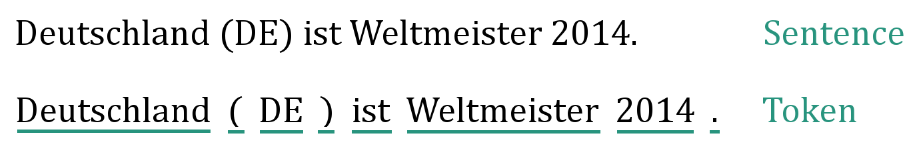
\includegraphics[width=0.6\linewidth]{./source/images/tokenization.png}}
  \caption{Tokenisierung eines beispielhaften Satzes.}
  \label{pic:Tokenization}
\end{figure}

\noindent
Die Arbeit mit Texten erfordert bekanntermaßen eine geeignete mathematische Form. Die zeichenbasierten Token der Texte werden daher in einem Wortschatz (engl. Vocabulary) mithilfe numerischer Indizes kodiert. Hier ist es möglich, die Anzahl eindeutiger Token zu identifizieren oder gar seltene Token aus praktischen Gründen zu entfernen \cite[S.~311-312]{ZHA20}.
\newpage

\noindent
Die Python-Bibliotheken \ac{NLTK} und SpaCy stellen entsprechende Tokenizer für eine möglichst schnelle Implementierung bereit. Beide sind überdies in einer für die deutsche Sprache ausgereiften Version verfügbar. Oftmals werden hierbei weitere Funktionalitäten mitgeliefert, darunter meist das Entfernen sprachbezogener Stoppwörter, die Lemmatisierung oder auch das Part-of-Speech-Tagging \cite[S.~111]{BIR09}.


\section{Word Embeddings}
\noindent
Algorithmen können Texte bekanntermaßen nicht in ihrer Rohform verarbeiten. Texte bedürfen einer geeigneten mathematischen Form. Word Embeddings überführen Texte oder ganze Korpora hierfür in einen Vektorraum (engl. Vector Space), um Wörter syntaktisch, semantisch und insbesondere untereinander in Kontext zu bringen. Dabei wird ein Wortschatz benutzt, welcher die entsprechenden Vektoren, bestehend aus eindeutig kodierbaren ganzzahligen Werten, aufbaut \cite{KAR18}. Die Ableitung der Vektoren aus den Textdaten wird auch als Feature Extraction oder Feature Encoding bezeichnet. Insgesamt befindet man sich hier im Bereich des Language Modeling \cite{BRO19}.\\

\noindent
Word Embeddings werden üblicherweise noch vor der Entwicklung der ursprünglich anvisierten \ac{NLP}-Aufgabe trainiert, weshalb ihnen ein unmittelbarer qualitativer Einfluss zugesprochen wird. Die entstehenden Modelle sind in der Folge schnell implementierbar. Weiterhin haben sie hiermit einen hohen skalierenden Effekt, da sie als Grundlage verschiedenster nachgelagerter \ac{NLP}-Aufgaben eingesetzt werden können \cite{NIT19}. Word Embeddings können durch verschiedene mehr oder minder komplexe Ansätze realisiert werden. Diese werden nachfolgend vorgestellt, wobei stets verdeutlicht wird, wie der entsprechende Vektorraum aufgebaut und in Kontext gebracht wird. Dabei wird außerdem deutlich, dass sich die verschiedenen Ansätze nicht für jede \ac{NLP}-Aufgabe eignen, sondern sie vielmehr einschränken. Obgleich nicht alle Ansätze für die \ac{ATS} relevant sein werden, sind sie als Grundlage zu verstehen.
\newpage


\subsection{One-Hot-Encoding}
\noindent
\ac{OHE} ist einer der einfachsten Ansätze, um Texte in einen Vektorraum einzubetten. Dabei werden allgemein kategorische Variablen in ein numerisches und somit mathematisch verarbeitbares Format gebracht \cite{KAR18}. Seien nun zwei gleichbedeutende Sätze gegeben. Eben jene Sätze sowie der entsprechende Wortschatz und die binär kodierten Vektoren sind in \autoref{pic:OneHotEncoding} ersichtlich. Die Vektoren sind hierbei als Matrix zusammengefasst, wobei die Zeilen und Spalten anhand der Anfangsbuchstaben der Wörter kenntlich gemacht sind.\\

\noindent
Versucht man nun, diese Vektoren in einem Vektorraum zu visualisieren, dann entspricht jeder Vektor einer eigenen Dimension. Dabei wird allerdings klar, dass keine dimensionsübergreifenden Projektionen existieren \cite{KAR18}. Dies bedeutet, dass die Wörter \textit{gutes} und \textit{schönes} genauso verschieden sind, wie die Wörter \textit{heute} und \textit{ist}. Dies ist offensichtlich falsch. \ac{OHE} ist dennoch als Grundlage zu verstehen, wobei etwaige Probleme innerhalb der nachfolgenden Ansätze weiterbehandelt werden.\\

\begin{figure}[h!]
  \centering
  \fbox{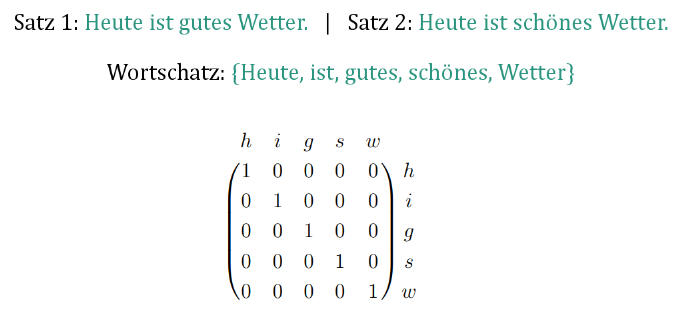
\includegraphics[width=0.65\linewidth]{./source/images/onehotencoding.png}}
  \caption{One-Hot-Encoding mit zwei beispielhaften Sätzen.}
  \label{pic:OneHotEncoding}
\end{figure}


\subsection{Bag-of-Words}
\noindent
\ac{BOW} realisieren die Feature Extraction, indem entsprechende Modelle das Aufkommen von in einem Wortschatz definierter Wörter über eine Vielzahl von Texten zählen. Dabei ist allerdings ein gewisser Informationsverlust zu erwarten, da beispielsweise die Reihenfolge der Wörter nicht berücksichtigt wird \cite[S.~262]{RAS19}. \autoref{table:BagOfWords} zeigt beispielhaft eine Matrix eines solchen \ac{BOW}-Modells.
\newpage

\noindent
In den Zeilen sind die betrachteten Texte indiziert, in den Spalten hingegen die Wörter des frei erfundenen Wortschatzes. Die Matrix hat demnach eine daran orientierte fixe Größe. In den Zellen ergeben sich somit die Häufigkeiten der Wörter, bezogen auf ihr Aufkommen in den einzelnen Texten \cite{BRO19}.

\begin{table}[htb]
\centering
\begin{tabular}{ | p{1.8cm} | p{1.8cm} | p{1.8cm} | p{1.8cm} | p{1.8cm} | p{1.8cm} | p{1.8cm} | p{1.8cm} | }
\hline
\textbf{ID} & \textbf{Vögel} & \textbf{sind} & \textbf{Tiere} & \textbf{der} & \textbf{Lüfte} \\
\hline
Text 1 & 2 & 8 & 1 & 5 & 1 \\
\hline
Text 2 & 1 & 3 & 0 & 2 & 0 \\
\hline
Text 3 & 0 & 4 & 0 & 7 & 0 \\
\hline
\end{tabular}
\caption{Bag-of-Words mit einem beispielhaften Wortschatz \cite{HUI20}.}
\label{table:BagOfWords}
\end{table}

\noindent
Nachteilig ist dieser Ansatz hinsichtlich der \ac{ATS} insbesondere dadurch, dass die Reihenfolge der Wörter nicht berücksichtigt wird. Wie in \autoref{table:BagOfWords} ersichtlich wurde, lassen sich aus der Matrix keine Informationen über die Semantik oder Grammatik rekonstruieren. Aus technischer Sicht würde die Matrix bei steigender Wortschatzgröße nicht nur mitwachsen, sondern zudem viele Null-Einträge enthalten \cite{HUI20}. Vorteilig ist dieser Ansatz hingegen für eher schlichtere \ac{NLP}-Aufgaben. Hier sei die Klassifikation von Dokumenten als mögliches Einsatzgebiet genannt.


\subsection{Skip-Gram-Model}
\noindent
Ein weiterer frequenzbasierter Ansatz besteht in sogenannten Skip-Gram-Modellen. Diese unterliegen der Annahme, dass sich der Kontext eines gegebenen Wortes in Form von einer Textsequenz generieren lässt. Sei hierfür nun beispielhaft und gleichermaßen abstrakt die Sequenz {\{\textit{a, b, c, d, e}\}} gegeben. Zudem sei \textit{c} das Zielwort und die lokale Fenstergröße zwei. Ein Skip-Gram-Modell modelliert die bedingten Wahrscheinlichkeiten für die vor- und nachstehenden Kontextwörter \cite[S.~640]{ZHA20}. Hierfür gilt die folgende Formel: $$P(a, b, d, e \mid c)$$

\noindent
Gemäß der weitergehenden Annahme, die Kontextwörter ließen sich auf Grundlage eines gegebenen Zielwortes unabhängig voneinander generieren, kann die Formel wie folgt umgeschrieben werden: $$P(a \mid c) \cdot P(b \mid c) \cdot P(d \mid c) \cdot P(e \mid c)$$
\newpage

\noindent
Sei darüber hinaus abstrakter Wortschatz gegeben. Dabei erfordert jedes darin enthaltene Wort zwei mehrdimensionale Vektoren. Einen, um das Wort als Zielwort zu evaluieren, und einen, um das Wort in den unterschiedlichen Kontexten einzuordnen. Mithilfe dieser Vektoren können die bedingten Wahrscheinlichkeiten des entsprechenden Modells trainiert werden. Autark ist jedoch auch dieser Ansatz ungeeignet für die \ac{ATS} \cite[S.~641]{ZHA20}.


\subsection{Word2Vec}
\noindent
Der Ansatz des \ac{W2V} kombiniert \ac{BOW}-Modelle mit Skip-Gram-Modellen, um die Nachteile des \ac{OHE} weitergehend aufzuarbeiten. Dabei werden \ac{BOW}-Modelle jedoch in kontinuierlicher Form genutzt. Diese funktionieren in umgekehrter Weise zu den Skip-Gram-Modellen. Damit ist folglich eine beidseitige Herangehensweise möglich. Der Kontext kann also aus einem gegebenen Zielwort und das Zielwort wiederum aus einem gegebenen Kontext ermittelt werden \cite[S.~644]{ZHA20}.\\

\noindent
Die entsprechenden bedingten Wahrscheinlichkeiten können gemäß der nachstehenden Formeln modelliert werden. Dabei werden Skip-Gram-Modelle (erstgenannt) den \ac{BOW}-Modellen (zweitgenannt) anhand des oben genannten Beispiels gegenübergestellt. $$P(a, b, d, e \mid c) \qquad P(c \mid a, b, d, e)$$

\noindent
\ac{W2V}-Modelle können mithilfe neuronaler Netze trainiert werden. Dies befähigt sie, Zusammenhänge zwischen Wörtern zu erlernen. Hierbei werden Distanzen minimiert, die aus den zuvor beschriebenen Vektoren hervorgehen. Dieser Ansatz eignet sich in der Folge etwa dazu, Synonyme für gegebene Wörter zu bestimmen. \ac{ATS}-Modelle, welche den \ac{W2V}-Ansatz verfolgen, konnten sich in der Vergangenheit bereits in akzeptablem Maße beweisen \cite{KAR18}.\\

\noindent
\autoref{pic:OnlineSphere} zeigt die beispielhaften Projektionen von etwa 10.000 Wörtern, welche mit dem Embedding Projektor von TensorFlow und einer entsprechenden Hauptkomponentenanalyse generiert wurden. Dabei ist das Ergebnis der Suche nach dem Wort $play$ zu sehen. Es ist erkennbar, dass bedeutungsähnliche Wörter kürzere Distanzen aufweisen.
\newpage

\begin{figure}[h!]
  \centering
  \fbox{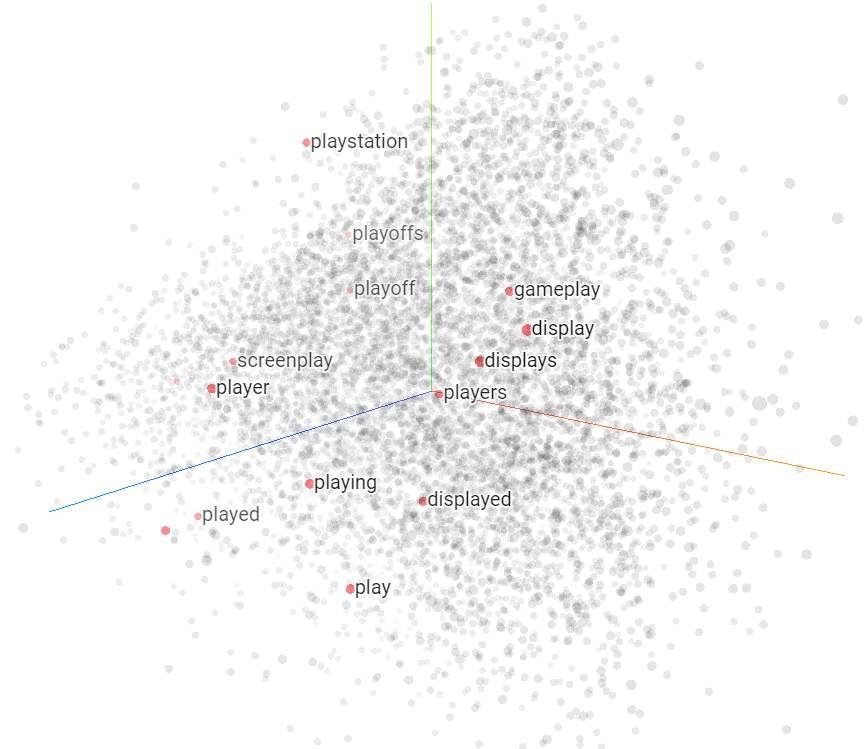
\includegraphics[width=0.75\linewidth]{./source/images/onlinesphere.png}}
  \caption{Word2Vec mit dem Embedding Projector von TensorFlow.}
  \label{pic:OnlineSphere}
\end{figure}


\subsection{Byte-Pair-Encoding}
\noindent
\ac{BPE} ist ein Algorithmus zur Datenkompression. Hierfür werden zusammenhängende Bytes mit einem Byte ersetzt, welches nicht in den sonstigen Daten auftritt \cite[S.~24]{NIT19}. Sei folgendes Beispiel gegeben: $$aaabcaacab = \boldsymbol{Z}\boldsymbol{Y}c\boldsymbol{Z}c\boldsymbol{Y}$$ $$\text{mit } \boldsymbol{Z} = aa \text{ und } \boldsymbol{Y} = ab$$

\noindent
\ac{BPE} eignet sich insbesondere dafür, seltene Wörter zu berücksichtigten. In diesen verbirgt sich mitunter eine nicht zu vernachlässigende Bedeutung. Aufgrund der kodierenden Funktion wird \ac{BPE} auch als Subword Embedding bezeichnet. Aufgrund der komprimierenden Funktion ist weiterhin von kleineren Modellgrößen auszugehen \cite[S.~24]{NIT19}. \ac{ATS}-Modelle, welche den \ac{W2V}-Ansatz verfolgen, konnten sich in der Vergangenheit ebenfalls in akzeptablem Maße beweisen.


\subsection{GloVe}
\noindent
\ac{GloVe} ist ein weiterer Algorithmus zur Einbettung von Texten in einen Vektorraum, welcher syntaktische und semantische Bedeutungen repräsentiert \cite[S.~1]{PEN14}.\\

\noindent
Hierfür wird sich einer Matrix bedient, welche das gemeinsame Aufkommen der im Korpus enthaltenen Wörter paarweise gegenüberstellt. Sie wird daher auch als Word-Word-Co-Occurrence-Matrix bezeichnet und besitzt eine maximale Komplexität von $O(|V|^2)$, wenn $V$ die Wortschatzgröße ist. \ac{GloVe} sieht dabei vor, die Matrix unter Nutzung lokaler Kontextfenster global zu faktorisieren \cite[S.~2]{PEN14}.\\

\noindent
Hierbei werden sehr große Matrizen durch mehrere niederrangige Matrizen approximiert. Dies ermöglicht es, die verborgenen statistischen Informationen des zugrundeliegenden Korpus anhand linearer Substrukturen zu explorieren und letztlich zu extrahieren. Dabei werden lokale Kontextfenster verwendet, wie sie bei verschiedenen oben genannten Ansätzen bereits beschrieben wurden, beispielsweise bei \ac{W2V} \cite[S.~24]{NIT19}.\\

\noindent
\ac{GloVe} ist praktisch als vortrainiertes Modell verfügbar. Dies basiert auf vier verschiedenen Korpora mit insgesamt etwa 55 Milliarden Token und einer durchschnittlichen Wortschatzgröße von etwa 1,5 Millionen Token. Im Training werden hierbei in der Matrix nur von Null verschiedene Werte berücksichtigt. Die mittlere quadratische Abweichung wird zudem als Fehlerfunktion ausgewählt. Das initiale Training ist zwar sehr rechenintensiv, dafür allerdings im Sinne des \ac{TL} a priori nur einmalig auszuführen. \ac{NLP}-Aufgaben, darunter auch die \ac{ATS}, profitierten stark vom Erfolg des \ac{GloVe}-Ansatzes. Trotzdem ist der Einsatz stets sorgfältig zu evaluieren, da innerhalb der modellinternen Vorverarbeitung die zugrundeliegenden Korpora beispielsweise auf Kleinschreibung forciert wurden. Dies müsste bei nachstehenden \ac{NLP}-Aufgaben ebenfalls berücksichtigt werden \cite[S.~6-9]{PEN14}.
\newpage


\section{Deep Language Representations}
\noindent
Die beschriebenen Word Embeddings verfolgen teils sehr abstrakte Ansätze, welche sich mitunter nur auf sehr wenige Teilbereiche des \ac{NLP} adaptieren lassen oder entscheidende Nachteile aufweisen. Zudem unterliegen sie meist statistischen und somit rechentechnischen Limitationen.\\

\noindent
\ac{ATS}-Modelle erfordern daher weitergehende Deep Language Representations, um den Anforderungen an das \ac{NLU} und die \ac{NLG} gerecht zu werden. Dabei werden die ursprünglichen Ansätze durch umfangreichere und komplexere neuronale Netze ersetzt. Diese werden fortan als Language Models bezeichnet. Nur wenige marktpräsente Akteure sind hierbei dazu fähig, geeignete Architekturen zu konzipieren und entsprechende Modelle von Grund auf neu zu trainieren. Dies wurde in der Vergangenheit bereits getan und veröffentlicht, sodass gemäß \ac{TL} nur noch ein weitergehendes Fine-Tuning nötig ist. Dabei profitierten nahezu alle nachstehenden \ac{NLP}-Aufgaben qualitativ von diesen Fortschritten. Architekturen, welche als Deep Language Representations zu verstehen sind und eine \ac{ATS} begünstigen, werden nachfolgend offengelegt \cite[S.~25]{NIT19}.


\subsection{ELMo}
\noindent
Zuerst sei \ac{ELMo} als Deep Contextualized Word Representation genannt. Es wurde vom Allen Institute for Artificial Intelligence entwickelt und 2018 veröffentlicht. \ac{ELMo} modelliert dabei einerseits komplexe Wortcharakteristiken wie Syntax und Semantik, andererseits aber auch den linguistischen Kontext eben dieser Wörter. Es ist als vortrainiertes Modell verfügbar und konnte nach der Veröffentlichung insbesondere \ac{NLU}-Aufgaben begünstigen \cite[S.~1]{PET18}.\\

\noindent
\ac{ELMo} arbeitet mit wortbezogenen kontextbasierten Vektoren, welche aus zwei bidirektionalen Language Models abgeleitet und trainiert werden. Diese bestehen wiederum aus zwei gekoppelten \ac{LSTM}-Schichten. Der umfangreiche Korpus an Textdaten wird dabei schichtweise vorwärts und rückwärts durch die Architektur propagiert. Somit sind kontextabhängige Informationen verfolgbar und die Bedeutungen der Wörter erlernbar. Aufgrund der zeichenbasierten Funktionsweise kann \ac{ELMo} sogar Wissen über Wortformen erlernen. Im Vergleich zu \ac{W2V} oder etwa \ac{GloVe} werden die Vektoren nicht tokenbasiert berechnet, sondern mithilfe einer Funktion, welche stets eine Sequenz berücksichtigt. Wörter können daher in verschiedenen Kontexten verschiedene Vektoren besitzen. \autoref{pic:ElmoStructure} visualisiert dies \cite[S.~2-3]{PET18}.

\begin{figure}[h!]
  \centering
  \fbox{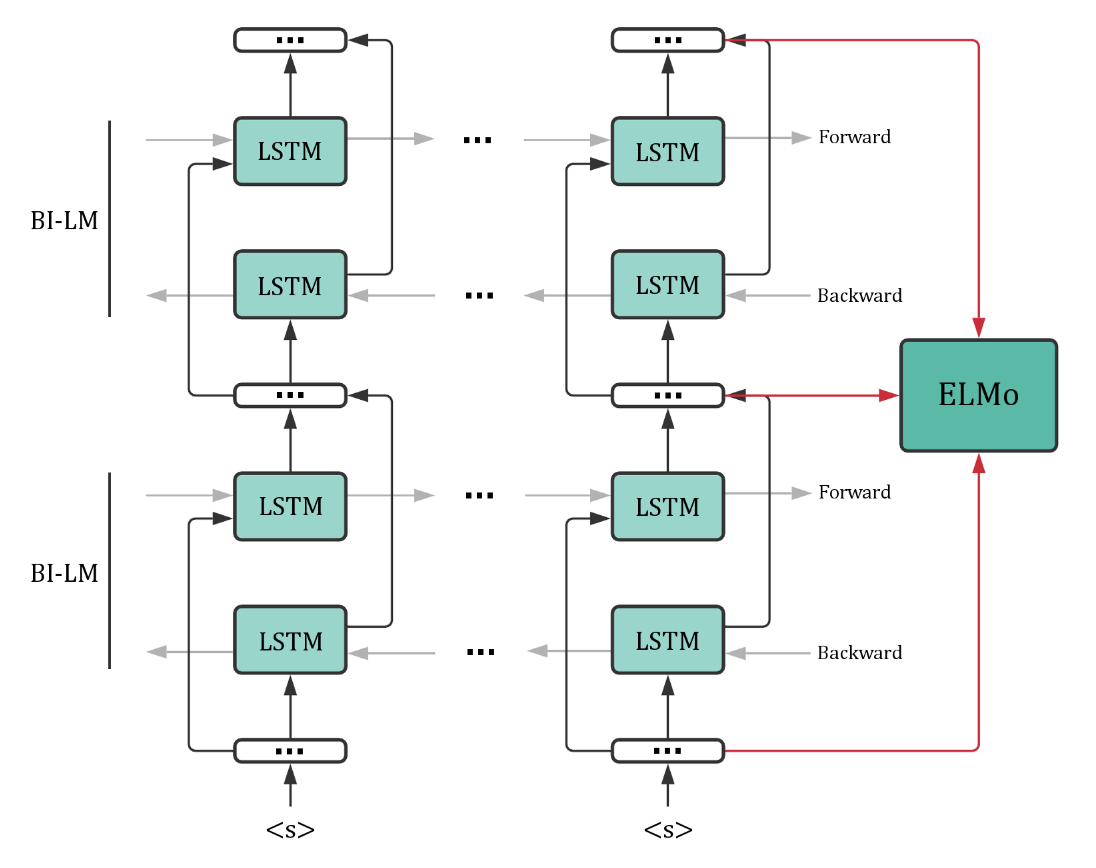
\includegraphics[width=0.7\linewidth]{./source/images/elmostructure.png}}
  \caption{Architektur und Funktionsweise von ELMo \cite{IRE18}.}
  \label{pic:ElmoStructure}
\end{figure}


\subsection{GPT}
\noindent
OpenAI arbeitet mit dem \ac{GPT} als Language Model in der nunmehr dritten Generation, veröffentlicht es allerdings nicht. Zu Forschungszwecken stellen sie dennoch eine schmalere Version des Modells bereit. OpenAI zeigt insbesondere mit dem \ac{GPT}, dass Language Models mithilfe der sogenannten Next Word Prediction besonders gut im Sinne des Unsupervised Learning trainiert werden können. Es basiert zudem auf der bereits bekannten Transformer-Architektur und begünstigt somit verschiedene nachgelagerte \ac{NLP}-Aufgaben, ohne entsprechende gelabelte Daten jemals gesehen zu haben. Dabei ist das \ac{GPT} meist besser als konkurrierende Modelle, welche auf den aufwendig zusammenzustellenden gelabelten Daten basieren, auch im sogenannten Zero-Shot-Transfer. Einer der größten Erfolge ist hierbei, dass das \ac{GPT} gemäß \ac{NLG} selbst einen Nachrichtenartikel verfassen konnte \cite[S.~1]{RAD19}.\\

\noindent
Die zugrundeliegenden Daten des \ac{GPT}-Modells bestehen aus 40GB an Texten, welche aus acht Millionen Internetseiten kollektiert wurden und zugleich bestimmten Qualitätsanforderungen gerecht werden. Hier nimmt OpenAI unter anderem an, dass Reddit-Beiträge mit einem ausreichend hohen positiven Karmastand eine erhöhte Qualität versprechen \cite[S.~3]{RAD19}.\\

\noindent
Im mathematischen Sinne wurde im Kontext der \ac{ATS} bislang meist die Wahrscheinlichkeit der Ausgabesequenz unter einer gegebenen Eingabesequenz modelliert. Language Models wie das \ac{GPT} streben hingegen ein allgemeineres Sprachverständnis an, um darüber hinaus eine Vielzahl an \ac{NLP}-Aufgaben unterstützen zu können. Daher modelliert das \ac{GPT} gemeinhin die Wahrscheinlichkeit $P(output \mid input, task)$ \cite[S.~2]{RAD19}. Aufgrund der eingeschränkten Verfügbarkeit seitens OpenAI entfallen an dieser Stelle weitere Ausführungen.


\subsection{BERT}
\noindent
Zuletzt sei \ac{BERT} als mögliches Modell zur Deep Language Representation genannt. Es wurde von Forschern der Google AI Language entwickelt und 2019 veröffentlicht. \ac{BERT} basiert auf ebenfalls der bereits bekannten Transformer-Architektur, wobei unstrukturierte Textdaten mithilfe links- und rechtsseitiger Kontextfenster bidirektional angelernt werden. Dabei entstammen die Daten verschiedenartigen \ac{NLP}-Aufgaben, sodass \ac{BERT} größtenteils aufgabenunabhängig einsetzbar ist. Im anschließenden Fine-Tuning werden die vortrainierten modellinternen Parameter zunächst initialisiert und wiederum mithilfe von gelabelten Daten angepasst. \ac{BERT} zeichnet sich weiterhin dadurch aus, dass er höchst anpassungsfähig ist und sich die vortrainierte Architektur nur minimal von der weitertrainierten Architektur unterscheidet \cite[S.~1-3]{DEV19}.\\

\noindent
Nun wird die Architektur von \ac{BERT} umfassender untersucht, indem die einleitenden Worte aufgegriffen und theoretisch ergründet werden. \ac{BERT} ist prinzipiell als Encoder zu verstehen, welcher durch einen mehrschichtigen bidirektionalen Transformer repräsentiert wird. Dabei werden die Schichten durch Transformer-Module repräsentiert. Diese verfügen über entsprechende Attention-Mechanismen, um kontextuelle Informationen zu erkennen. Weiterhin werden Sequenzen nicht nur einseitig betrachtet, sondern beidseitig, also bidirektional. Somit werden wortbezogene Kontexte gelernt, was insbesondere zu einem tieferen Verständnis der Sprache seitens \ac{BERT} führt. Dies ist ein großer Vorteil gegenüber bisheriger Architekturen, inklusive \ac{ELMo} und \ac{GPT}, welche Sequenzen zumeist nur einseitig betrachten konnten, also von links nach rechts oder andersherum. Aufgrund der qualitativen Vorteile von \ac{BERT} wird es umfänglicher als die ausgewählten Vorgänger und Konkurrenten analysiert \cite[S.~3]{DEV19}.
\newpage

\noindent
Um \ac{BERT} entsprechend vortrainieren zu können, werden \ac{MLM} genutzt. Bevor die Textdaten in die Architektur geführt werden, werden etwa 15\% der Wörter durch ein $[\text{MASK}]$-Token ersetzt. Daraufhin versucht das Modell, die maskierten Token auf Grundlage der umliegenden nicht-maskierten Token vorherzusagen (engl. Next Word Prediction). Da die zu erwartenden Wörter bekannt sind, kann über eine Klassifikationsschicht ein Lerneffekt erzielt werden, indem entsprechende Matrizen dimensional transformiert und wertmäßig aktualisiert werden. \autoref{pic:BertEncoder} zeigt die beschriebene Architektur \cite[S.~4-5]{DEV19}.\\

\begin{figure}[h!]
  \centering
  \fbox{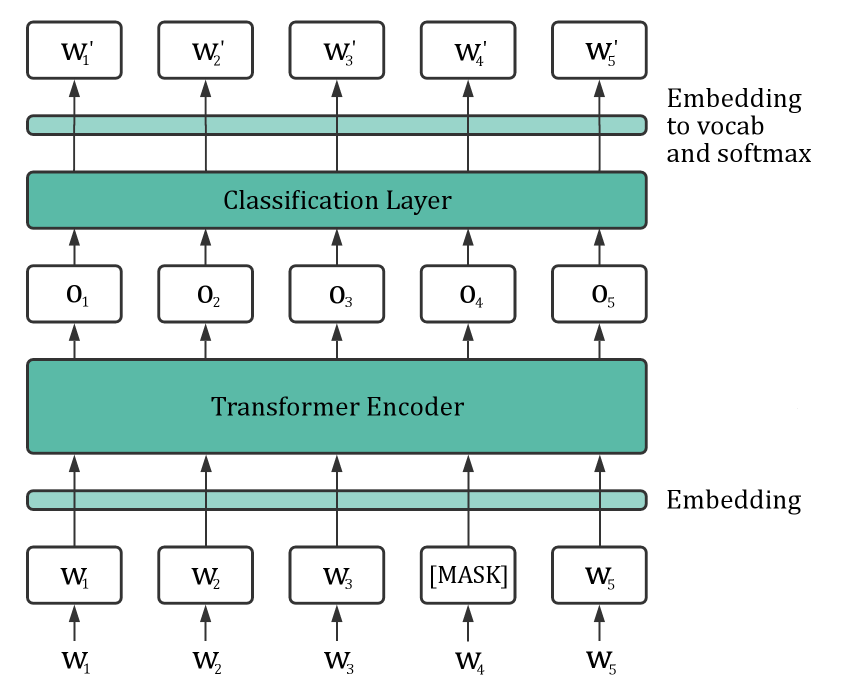
\includegraphics[width=0.65\linewidth]{./source/images/bertencoder.png}}
  \caption{Architektur von BERT mit MLM \cite[S.~3]{DEV19}.}
  \label{pic:BertEncoder}
\end{figure}

\noindent
Um zudem weitergehende Informationen auf Satzebene zu erhalten, werden dem Training paarweise Sätze zugeführt. Seien $A$ und $B$ zwei solcher Sätze, dann ist $B$ zu 50\% ein auf $A$ folgender Satz und zu 50\% ein zufälliger Satz des Korpus. Dies wird erneut im Sinne einer Klassifikation gelernt (engl. Next Sentence Prediction). Wie \ac{BERT} die eingehenden Sequenzen einbettet und repräsentiert, wird in \autoref{pic:InputRepresentation} deutlich. Dabei handelt es sich um die Summe der Token Embeddings, Segment Embeddings und Position Embeddings. Hierbei kann entschieden werden, ob Klein- und Großschreibung berücksichtigt werden soll \cite[S.~3-5]{DEV19}.
\newpage

\begin{figure}[h!]
  \centering
  \fbox{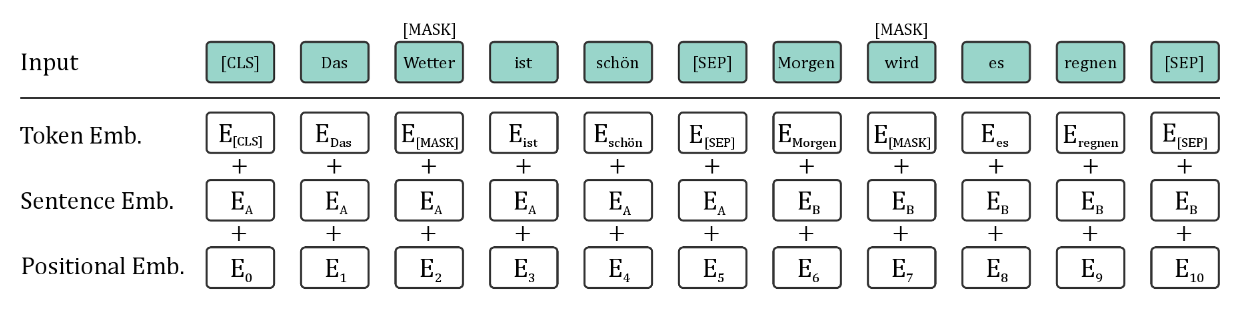
\includegraphics[width=0.95\linewidth]{./source/images/inputrepresentation.png}}
  \caption{Repräsentation von Textdaten mithilfe von BERT \cite[S.~3]{DEV19}.}
  \label{pic:InputRepresentation}
\end{figure}

\noindent
\ac{BERT} wurde initial in zwei verschiedenen Versionen veröffentlicht: BASE und LARGE. Die veröffentlichten Modelle wurden von den Forschern der Google AI Language auf zwei verschiedenen Korpora mit insgesamt über drei Millionen Wörtern trainiert. Sei $L$ die Anzahl der Schichten (oder: Transformer-Module), $H$ die Größe der verborgenen Schichten und $A$ die Anzahl der Self-Attention-Heads, dann sind die Versionen wie folgt definiert \cite[S.~3-5]{DEV19}. $$\text{BERT}_{\text{BASE}}: (L=12, H=768, A=12) \text{ mit } 110 \text{M Parametern}$$ $$\text{BERT}_{\text{LARGE}}: (L=24, H=1024, A=16) \text{ mit } 340 \text{M Parametern}$$

\cleardoublepage

\chapter{Datengrundlage}
\thispagestyle{fancy}
\label{chap:Datengrundlage}

\noindent
Um die Ziele dieser Arbeit zu erreichen, ist die Entwicklung theoretisch analysierter Architekturen zur \ac{ATS} und zur sprachtechnischen Adaption erforderlich. Hierfür ist eine geeignete Datengrundlage bereitzustellen, welche insbesondere Qualität, aber auch Vergleichbarkeit der entsprechenden Modelle ermöglicht. Fortan wird die Datengrundlage als Korpus $K$ bezeichnet, wobei dieser Korpus aus verschiedenen Datensätzen $d_i$ besteht, also $$K=\begin{pmatrix} d_1 \\ \vdots \\ d_n \end{pmatrix}$$ für $i=1,...,n$ mit möglichst großem $n$ hinsichtlich hoher Qualität. Die Datensätze, welche den gesuchten Korpus bilden, müssen dabei bestimmten Anforderungen genügen. Ihnen wird insbesondere eine paarweise Natur abverlangt. Für $d_i \in K$ und $i=1,...,n$ gilt also: $d_i=\{t_i,s_i\}$. Neben dem ursprünglichen Text $t_i$ ist hier eine Zusammenfassung $s_i$ gefordert, welche als Referenz für die modellseitig zu generierende Zusammenfassung dient. Nur so ist die Qualität messbar und der Lernfortschritt realisierbar. Aufgrund der explorativen Natur dieser Arbeit werden sowohl englischsprachige als auch deutschsprachige Datensätze benötigt, wobei deren zugrundeliegende Domäne zunächst nicht von hoher Relevanz ist. Die Länge der Texte und der Zusammenfassungen haben einen hohen Einfluss darauf, wie das trainierte Modell die eigenen Zusammenfassungen generieren wird. Zwar wird hierfür keine Mindestlänge definiert, dennoch seien folgende Richtwerte gegeben: Texte $t_i$ sollten aus mindestens 200 Wörtern bestehen. Zusammenfassungen $s_i$ hingegen sollten einige Sätze vorweisen können. Alle Texte und Zusammenfassungen sollten zwischen Klein- und Großschreibung unterscheiden.\\

\noindent
Unter Berücksichtigung obiger Anforderungen werden nun drei Korpora ausgewählt. Der erste Korpus dient als initialer Trainingskorpus und besteht aus etwa 300.000 englischsprachigen Datensätzen. Er wurde von TensorFlow verarbeitet und veröffentlicht, entstammt allerdings ursprünglich der CNN und der DailyMail \cite{TEN21}. Aufgrund der nachrichtenorientierten Domäne ist von stark variierenden Textinhalten auszugehen. Dies verspricht zunächst einen hohen generalisierenden Effekt, wobei andere Domänen wiederum andere Eigenarten aufweisen und mitunter eine andere Beschaffenheit des Korpus erfordern. Dies ist allerdings nicht Teil dieser Arbeit und gilt lediglich als sensibilisierende Anmerkung. Die Eignung des Korpus wird insbesondere durch die weitreichende Nutzung in der Wissenschaft bestärkt, denn \ac{SOTA}-Modelle werden oftmals auf diesem Korpus verglichen. Texte dieses Korpus bestehen durchschnittlich aus etwa 850 Wörtern, Zusammenfassungen hingegen aus etwa 60 Wörtern. Dies spricht für einen hohen Abstraktionsgrad und damit eine hohe Verdichtung \cite[S.~6]{ROT20}.\\

\noindent
Die anderen beiden Korpora dienen dem weitergehenden Training hinsichtlich der sprachtechnischen Adaption und bestehen demzufolge aus deutschsprachigen Datensätzen. Der erste Korpus hiervon wurde 2019 im Kontext der Swiss Text Analytics Conference als Grundlage eines Wettbewerbes publiziert und umfasst 100.000 Datensätze \cite{CIE19}. Die Textinhalte entstammen der deutschsprachigen Wikipedia, weshalb auch hier von einer vielfältigen Domäne auszugehen ist. Letzteres gilt auch für den zweiten Korpus, welcher durch einen in Python selbst entwickelten Crawler generiert wurde. In einer Zeitspanne von sechs Monaten wurden mehr als 50.000 Nachrichtenartikel automatisiert kollektiert \cite[S.~79,~83,~416]{BIR09}. Nach Sichtung der verfügbaren Daten können Artikel der ZEIT ONLINE als geeignet bewertet werden. Demnach sind etwa 15.000 Datensätze nutzbar. Texte dieser beiden Korpora bestehen durchschnittlich aus etwa 4.000 Wörtern, Zusammenfassungen hingegen aus etwa 250 Wörtern. Üblicherweise existiert beim anvisierten Training die Gefahr der sogenannten Exploitation. Diese Gefahr meint im Kontext der \ac{ATS} konkret, dass das zugrundeliegende Modell die Struktur der Artikel anstatt der Inhalte der Artikel lernt. Grund für diese Annahme ist der typische Aufbau von Wikipedia-Artikeln. Diese beinhalten zumeist bereits im ersten Absatz stark verdichtete Informationen, also eine Art Zusammenfassung. Daher wird zur Vorbeugung eine Mischung aus den beiden deutschen Korpora vorgenommen \cite[S.~42]{BIR09}.\\

\cleardoublepage

\chapter{Abstraktiver Ansatz}
\thispagestyle{fancy}
\label{chap:Abstraktiver Ansatz}

Notizen:
\begin{itemize}
	\item Abgrenzung zum extraktiven Ansatz beschreiben
	\item Vorteile gegenüber referenzierten Modellen herausstellen
	\item Generierung neuer Sätze sowohl mit vorkommenden als auch mit nicht-vorkommenden Wörtern (vgl. Paper: „Automatic Text Summarization with Machine Learning“)
	\item BERT: \url{https://towardsdatascience.com/summarization-has-gotten-commoditized-thanks-to-bert-9bb73f2d6922}
	\item Siehe Abstract im Exposé
\end{itemize}


\section{Architektur}
Notizen:
\begin{itemize}
	\item Netzwerk des abstraktiven Ansatzes als Pipeline skizzieren
\end{itemize}


\section{Konfiguration}
Notizen:


\section{Training}
Notizen:
\begin{itemize}
	\item Training verschiedener Modelle
\end{itemize}


\section{Evaluation}
Notizen:
\begin{itemize}
	\item Kompressionsrate messen
	\item Qualität der Zusammenfassung messen
	\item Evaluation verschiedener Modelle mit geeigneter Vergleichstabelle
	\item Vergleich mit SOTA-Modellen
	\item Praktische Nutzung durch Implementation eines vortrainierten Modells in ein Skript oder eine Software
\end{itemize}

\cleardoublepage

\chapter{Sprachtechnische Adaption}
\thispagestyle{fancy}
\label{chap:Sprachtechnische Adaption}

\noindent
Unter Kenntnis der Architektur des abstraktiven Ansatzes und der Baseline des englischsprachigen Modells wird nun ergründet, wie eine Adaption auf die deutsche Sprache erfolgen kann. Dies wird mithilfe verschiedener Experimente erprobt, welche sich weiterhin auf die bekannten Metriken stützen.


\section{Architektur}
\noindent
Die bislang genutzte Architektur, welche bekanntermaßen Transformer integriert, kann auf Grundlage umfangreicher verschiedensprachiger ungelabelter Textdaten im Sinne des \ac{DL} und \ac{TL} multilingual vortrainiert werden, ohne architektonische Anpassungen vornehmen zu müssen. Hierbei werden sprachübergreifende verborgene Strukturen erlernt, um anschließend monolingual davon zu profitieren. Zudem wird dem Problem entgegengewirkt, dass sprachintern zu wenig Textdaten zur Verfügung stehen \cite{MOB20}. Modelle, welche organisationsextern bereits multilingual vortrainiert und bereitgestellt wurden, sind beispielsweise die multilinguale Version von \ac{BERT} und die \ac{XLM-R}. Hinsichtlich einer anschließenden deutschsprachigen Nutzung in der \ac{ATS} ist weiterhin ein entsprechendes sprachbezogenes Training erforderlich. Dies wird im Verlauf der Experimente hinreichend abgehandelt.


\section{Experimente}
\noindent
In einem initialen Experiment wird die multilinguale Version von \ac{BERT} mit einem Mix aus allen verfügbaren deutschsprachigen Daten trainiert. Hierbei entstehen die folgenden \ac{ROUGE}-Scores: R-Recall: 24.56, R-Precision: 15.05, R-Measure: 17.25. Dies überliegt dem \ac{SOTA} zwar deutlich, ist allerdings auf die Struktur der Trainingsdaten zurückzuführen, da mehr als die Hälfte aller Daten aus Wikipedia-Artikeln stammen.
\newpage

\noindent
Dennoch sei nachfolgend die Zusammenfassung des in Anhang B einzusehenden deutschsprachigen Textes gezeigt. Dieser gleicht strukturell sowie inhaltlich dem bereits beschriebenen Text in Anhang A. In der Folge schließen sich verschiedene jeweils aus dem vorherigen Schritt abgeleitete Experimente an.\\

\noindent\fbox{%
\parbox{\textwidth}{%
In New York ist ein Flugzeug aus dem World Trade Center auf dem Nordturm des World Trade Centers gebrannt. In den USA ist es zu einem Unfall gekommen. Nun ist das Land wieder in Schock, wo es sich um einen Brand ereignete. Es war der erste Unfall, der sich in den USA ereignet hat.
}%
}\\

\noindent
Die inhaltliche Schwäche ist für den menschlichen Leser unschwer erkennbar auch ohne Kenntnis über den Originaltext. Daher wird nun die multilinguale Version von \ac{BERT} durch eine eigens für die deutsche Sprache vortrainierte Version ausgetauscht. An der deutschsprachigen Datengrundlage wird zunächst nichts verändert. Hierbei entstehen die folgenden \ac{ROUGE}-Scores: R-Recall: 24.20, R-Precision: 14.65, R-Measure: 16.85. Dies unterliegt den \ac{ROUGE}-Scores der multilingualen Version von \ac{BERT}. Letzterer scheint tatsächlich von den verborgenen Strukturen anderer Sprachen zu profitieren.\\

\noindent
Mit dem Wissen, dass multilingual vortrainierte Modelle sogar die Qualität monolingualer Modelle im deutschsprachigen Raum übersteigen, wird nun \ac{BERT} durch \ac{XLM-R} ersetzt, um sich geeigneten Ergebnissen zu nähern. Es entstehen die folgenden \ac{ROUGE}-Scores: R-Recall: 0.00, R-Precision: 0.00, R-Measure: 0.00. TODO: KRITIK UND DEUTSCHE ZUSAMMENFASSUNG, WAHRSCHEINLICH NUTZUNG VON XLM-R BEGRÜNDEN, WEITERHIN STRUKTUR ERLERNT, DAHER UNTEN METHODISCH WEITER.\\

\noindent\fbox{%
\parbox{\textwidth}{%
Lorem ipsum dolor sit amet, consetetur sadipscing elitr, sed diam nonumy eirmod tempor invidunt ut labore et dolore magna aliquyam erat, sed diam voluptua. At vero eos et accusam et justo duo dolores et ea rebum. Stet clita kasd gubergren, no sea takimata sanctus est Lorem ipsum dolor sit amet. Lorem ipsum dolor sit amet, consetetur sadipscing elitr, sed diam nonumy eirmod tempor invidunt ut labore et dolore magna aliquyam erat, sed diam voluptua. At vero eos et accusam et justo duo dolores et ea rebum. Stet clita kasd gubergren, no sea takimata sanctus est Lorem ipsum dolor sit amet. Lorem ipsum dolor sit amet, consetetur sadipscing elitr, sed diam nonumy eirmod tempor invidunt ut labore et dolore magna aliquyam erat, sed diam voluptua. At vero eos et accusam et justo duo dolores et ea rebum. Stet clita kasd gubergren, no sea takimata sanctus est Lorem ipsum dolor sit amet.
}%
}\\

\noindent
Um den Umfang der deutschsprachigen Datengrundlage nicht reduzieren zu müssen, wird nun zunächst der jeweils erste Abschnitt der Wikipedia-Artikel entfernt. Ein erneutes Training der \ac{XLM-R} bringt die folgenden \ac{ROUGE}-Scores hervor: R-Recall: 0.00, R-Precision: 0.00, R-Measure: 0.00. TODO: KRITIK BZGL. OVERFITTING. Die entstehende Zusammenfassung sieht nun wie folgt aus:\\

\noindent\fbox{%
\parbox{\textwidth}{%
Lorem ipsum dolor sit amet, consetetur sadipscing elitr, sed diam nonumy eirmod tempor invidunt ut labore et dolore magna aliquyam erat, sed diam voluptua. At vero eos et accusam et justo duo dolores et ea rebum. Stet clita kasd gubergren, no sea takimata sanctus est Lorem ipsum dolor sit amet. Lorem ipsum dolor sit amet, consetetur sadipscing elitr, sed diam nonumy eirmod tempor invidunt ut labore et dolore magna aliquyam erat, sed diam voluptua. At vero eos et accusam et justo duo dolores et ea rebum. Stet clita kasd gubergren, no sea takimata sanctus est Lorem ipsum dolor sit amet. Lorem ipsum dolor sit amet, consetetur sadipscing elitr, sed diam nonumy eirmod tempor invidunt ut labore et dolore magna aliquyam erat, sed diam voluptua. At vero eos et accusam et justo duo dolores et ea rebum. Stet clita kasd gubergren, no sea takimata sanctus est Lorem ipsum dolor sit amet.
}%
}\\

\noindent
- Sliding-Window-Approach bei zu großen Texten beschreiben und entwickeln, Zielgröße von 512 anvisieren\\

\noindent
- Wikipedia-Anteil reduzieren
- XLM-R auf Wikipedia trainieren, nur auf ZEIT evaluieren
- XLM-R auf ZEIT trainieren und evaluieren\\

\noindent
- Alternative: BERT zur Translation nutzen, CNN/ Dailymail übersetzen\\
- Option: XLM-RoBERTa BASE/ LARGE, evtl. zu wenig Daten, dann auf vielversprechenden Fortschritt verweisen, (\url{https://huggingface.co/transformers/model_doc/xlmroberta.html})\\
- Option: Electra (\url{https://huggingface.co/german-nlp-group/electra-base-german-uncased})\\
- Option: BART von Facebook, multilingual (\url{https://huggingface.co/facebook/mbart-large-cc25})
- Optionen entweder in der Theorie ergänzen oder hier eingangs erwähnen

\noindent
-> Kapitel besser strukturieren (format-technisch, inhaltlich)
-> Beschreibung der Datengrundlage nochmal überprüfen
-> Lorem ipsum und Capslock-TODO's in beiden Kapiteln herausarbeiten 
-> Hyperparameteroptimierung auf 10-20 Prozent der Daten\\
-> Verdichtung der Zusammenfassung verdeutlichen, d.h. Token-Reduktion, zudem die prozentuale Kompressionsrate angeben, d.h. mit technischen Anpassungen können auch 5 DIN A4-Seiten um x Prozent verdichtet werden (Wie lang ist der Eingangstext? Wie lang ist der Ausgangstext?
Wie geht das Modell mit längeren Texten um?)

\noindent
+ \cite{YAN19} S. 4 rechts, Herausforderung: Encoder overfitted, Decoder underfitted oder andersherum, wird durch HuggingFace-Framework vorgebeugt
+ \cite{YAN19} S. 5 oben für Evaluation
+ Vergleichstabelle der Experimente einbinden und beschreiben
+ Typisches Diagramm zur Visualisierung des Trainingsprozesses anfügen
+ Verhalten des Modells interpretieren und Anpassungen ableiten, bspw. Exploitation wegen der Struktur der Artikel nochmal aufgreifen, ggf. erst bei der sprachtechnischen Adaption
+ Erwähnen, dass dies als Experiment genügt, sprachtechnische Anpassungen dann erst im nächsten Kapitel
+ Referenzzusammenfassungen mit ROUGE und BLEU bewerten, um Vergleichswerte nennen zu können
+ Texte manuell zusammenfassen, um ebenfalls einen Vergleichswert von ROUGE und BLEU zu haben\\

\cleardoublepage

\chapter{Zusammenfassung}
\thispagestyle{fancy}
\label{chap:Zusammenfassung}

\noindent
In dieser Arbeit wurde die Adaption multilingual vortrainierter Modelle zur automatischen Zusammenfassung von Texten auf die deutsche Sprache erforscht und demonstriert. Hierfür wurden entsprechende Grundlagen in \ac{DL} und \ac{NLP} offengelegt. Dabei ist insbesondere der kontextbezogene Fortschritt durch \ac{TL} in Assoziation mit den eingeführten \ac{DLR} hervorzuheben. Um das Ziel dieser Arbeit zu erreichen und die Forschungsfragen hinreichend zu beantworten, schlossen sich verschiedene Experimente an, deren Architektur und Datengrundlage zuvor methodisch aufbauend definiert wurde.\\

\noindent
Das Ziel dieser Arbeit, multilingual vortrainierte Modelle mittels \ac{TL} auf die deutsche Sprache zu adaptieren, konnte mithilfe von \ac{TF2TF} unter Nutzung von \ac{BERT} und \ac{BART} erreicht werden. Die entsprechenden Architekturen erreichen den \ac{SOTA} der \ac{ATS} in Englisch sowie in Deutsch. Die analysierten qualitativen Schwächen sind jeweils mit existierenden \ac{SOTA}-Modellen vergleichbar und daher akzeptabel. Hierbei ist außerdem anzumerken, dass mit HuggingFace selbst eines der größten Unternehmen der Branche, welches theoretisch über entsprechende Ressourcen verfügt, keine optimalen Ergebnisse erzielt. Es folgt die Beantwortung der einleitend formulierten Forschungsfragen.
\newpage

\noindent
\textbf{Wie lassen sich Texte automatisiert zusammenfassen?}\\
\noindent
Hierfür bedarf es einer Architektur, welche die Grundlagen des \ac{NLP} vereint, entsprechend vortrainierte \ac{DLR} integriert und ein weitergehendes Fine-Tuning auf möglichst vielen paarweisen Textdaten ermöglicht, um die Herausforderungen des \ac{NLU} und der {NLG} zu bewältigen. Dies wird beispielsweise von einem Sequence-to-Sequence-Transformer-Modell, welches über einen Encoder und einen Decoder verfügt, erfüllt.\\

\noindent
\textbf{Wie können existierende Modelle auf eine andere Sprache adaptiert werden?}\\
\noindent
Hierfür sind nicht zwingend architektonische Anpassungen notwendig, sondern vielmehr ein Austausch der Textdaten auf die entsprechende Zielsprache. Die oben beschriebene Architektur ist folglich in der Lage, sprachabhängige Strukturen dynamisch zu erlernen. Dabei wird die Qualität der Adaption entscheidend von den zugeführten Textdaten beeinflusst. Hier wird im folgenden Kapitel hinreichend angeknüpft.\\

\noindent
\textbf{Wie qualitativ und skalierbar ist die Lösung?}\\
\noindent
Während die untersuchten Architekturen wertmäßig den \ac{SOTA} erreichen, konnten qualitativ verschiedene Eigenarten identifiziert werden. Dies ist jedoch meist nicht den Architekturen selbst anzurechnen, sondern den zugeführten Textdaten, da sich die Architekturen in anderen Sprachen mit entsprechend umfangreichen und qualitativen Textdaten bereits bewährt haben. Daher ist gleichermaßen nicht davon auszugehen, dass die Architekturen größere Probleme mit der deutschen Sprache haben. Wurde ein Modell erst einmal hinreichend trainiert, kann es veröffentlicht, in Anwendungen implementiert und somit entsprechend skaliert werden. Hierbei ist das Echtzeitverhalten jedoch hinreichend zu analysieren, insofern dies im Anwendungsfall relevant ist.

\cleardoublepage

\chapter{Diskussion und Ausblick}
\thispagestyle{fancy}
\label{chap:Diskussion und Ausblick}

% TODO: Adaptive Learning für die Modelle ansatzweise vorstellen, Modell auf Dialogcharakter adaptieren, um es in der Verdichtung von Protokollen einer Videosprechstunde zu nutzen, bzw. generell bspw. Meetings zusammenzufassen, Forschungsstand und SOTA-Modelle hierfür im einleitenden Kapitel beschreiben, hier aufgreifen (vgl. Paper: „Abstractive Dialogue Summarization with Sentence-Gated Modeling Optimized by Dialogue Acts“ und “Using a KG-Copy Network for Non-Goal Oriented Dialogues”), bereits Architekturen vorstellen (vgl. „Automatic Dialogue Summary Generation of Customer Service“ und „Dialogue Response Generation using Neural Networks and Background Knowledge“ und „Global Summarization of Medical Dialogue by Exploiting Local Structures”), Modell ohne Anpassungen auf Konversationen anwenden: \url{https://www.isi.edu/natural-language/people/hovy/papers/05ACL-email_thread_summ.pdf}, Modell nutzen, um Zusammenfassungen für Texte zu generieren und damit neue Datensätze für neue Modelle zu generieren, aber stark von der Qualität abhängig, gelb markierte Literatur sichten und verwenden, Datumsangaben aktualisieren, Ausblick: Zusammenfassungen formatieren, also Großschreibung nach Satzenden oder auch Leerzeichenentfernung vor Punkten, Adaption auf Sprache und/ oder Domain, Ausblick: Ausblick: Datengrundlage besteht aus frei verfügbaren allgemeinsprachlichen, ausreichend langen und deutschsprachigen Daten, verschiedene Herkünfte, auf Grundlage dieser Allgemeinsprache und den eben genannten Vorhaben, sollte ein grundlegendes Modell trainiert werden und später für den Use Case eine Art Adaptive Learning betrieben werden, d.h. wenn bekannt ist, dass das Modell für medizinische Texte angewandt werden soll, sollte man vorher die Parameter des Modells finetunen, Gefahr: Initial bereits hohe Informationsdichte bei Diktaten - "Was fällt raus?", Ausblick: Limitations von NLP: \cite[S.~30-31]{BIR09}, Fine-Tuning in Zieldomäne notwendig

\cleardoublepage
\renewcommand{\baselinestretch}{1.0}
\small

\addcontentsline{toc}{chapter}{Literaturverzeichnis}
\setcounter{page}{85}

\begin{thebibliography}{85}
\thispagestyle{fancy}

\bibitem[AI-United, 2019]{AIU19}
AI-United: LSTM als neuronales Netzwerk mit langem Kurzzeitgedächtnis, in: \url{http://www.ai-united.de/lstm-als-neuronales-netzwerk-mit-langem-kurzzeitgedaechtnis/}, Aufruf am 23.04.2021.

\bibitem[Arbel, 2018]{ARB18}
Arbel, Nir: How LSTM Networks Solve the Problem of Vanishing Gradients, in: \url{https://medium.datadriveninvestor.com/how-do-lstm-networks-solve-the-problem-of-vanishing-gradients-a6784971a577}, Aufruf am 23.04.2021.

\bibitem[Beltagy et al., 2020]{BEL20}
Beltagy, Iz \& Peters, Matthew \& Cohan, Arman: Longformer as the Long-Document Transformer, Allen Institute for Artificial Intelligence, Seattle, 2020.

\bibitem[Bird et al., 2009]{BIR09}
Bird, Steven \& Klein, Ewan \& Loper, Edward: Natural Language Processing with Python, Verlag O'Reilly, Sebastopol, Vereinigte Staaten, 2009.

\bibitem[Brownlee, 2019]{BRO19}
Brownlee, Jason: A Gentle Introduction to the Bag-of-Words Model, in: \url{https://machinelearningmastery.com/gentle-introduction-bag-words-model/}, Aufruf am 19.05.2021.

\bibitem[Cieliebak, 2019]{CIE19}
Cieliebak, Mark: German Text Summarization Challenge, Swiss Text Analytics Conference, Winterthur, 2019.

\bibitem[Conneau et al., 2020]{CON20}
Conneau, Alexis \& Khandelwal, Kartikay \& Goyal, Naman \& Chaudhary, Vishrav \& Wenzek, Guillaume \& Guzman, Francisco \& Grave, Edouard \& Ott, Myle \& Zettlemoyer, Luke \& Stoyanov, Veselin: Unsupervised Cross-Lingual Representation Learning at Scale, Facebook AI, 2020.

\bibitem[CS231N, O. J.]{CSNOJ}
Convolutional Neural Networks for Visual Recognition: Nesterov Momentum, in: \url{https://cs231n.github.io/neural-networks-3/}, Aufruf am 16.04.2021.

\bibitem[Culurciello, 2018]{CUR18}
Culurciello, Eugenio: The Fall of RNN/ LSTM, in: \url{https://towardsdatascience.com/the-fall-of-rnn-lstm-2d1594c74ce0}, Aufruf am 23.04.2021.

\bibitem[Devlin et al., 2019]{DEV19}
Devlin, Jacob \& Chang, Ming-Wei \& Lee, Kenton \& Toutanova, Kristina: Pre-training of Deep Bidirectional Transformers for
Language Understanding, Google AI Language, 2019.

\bibitem[Ding et al., 2020]{DIN20}
Ding, Ming \& Zhou, Chang \& Yang, Hongxia \& Tang, Jie: Applying BERT to Long Texts, in: \url{https://proceedings.neurips.cc/paper/2020/file/96671501524948bc3937b4b30d0e57b9-Paper.pdf}, Aufruf am 26.05.2021.

\bibitem[Edpresso, O. J.]{EDPOJ}
Edpresso: Overfitting and Underfitting, in: \url{https://www.educative.io/edpresso/overfitting-and-underfitting}, Aufruf am 09.04.2021.

\bibitem[Gambhir et al., 2016]{GAM16}
Gambhir, Mahak \& Gupta, Vishal: Recent Automatic Text Summarization Techniques, University of Panjab in Chandigargh, 2016.

\bibitem[Goncalves, 2020]{GON20}
Goncalves, Luis: Automatic Text Summarization with Machine Learning, in: \url{https://medium.com/luisfredgs/automatic-text-summarization-with-machine-learning-an-overview-68ded5717a25}, Aufruf am 16.03.2021.

\bibitem[HuggingFace, 2021]{HUG21}
HuggingFace: The AI community building the future, in: \url{https://huggingface.co/}, Aufruf am 14.06.2021.

\bibitem[Huilgol, 2020]{HUI20}
Huilgol, Purva: Quick Introduction to Bag-of-Words (BoW) and TF-IDF for Creating Features from Text, in: \url{https://www.analyticsvidhya.com/blog/2020/02/quick-introduction-bag-of-words-bow-tf-idf/}, Aufruf am 19.05.2021.

\bibitem[Irene, 2018]{IRE18}
Irene: ELMo in Practice, in: \url{https://ireneli.eu/2018/12/17/elmo-in-practice/}, Aufruf am 26.05.2021.

\bibitem[Karani, 2018]{KAR18}
Karani, Dhruvil: Introduction to Word Embedding and Word2Vec, in: \url{https://towardsdatascience.com/introduction-to-word-embedding-and-word2vec-652d0c2060fa}, Aufruf am 19.05.2021.

\bibitem[Karim, 2019]{KAR19}
Karim, Raimi: Self-Attention, in: \url{https://towardsdatascience.com/illustrated-self-attention-2d627e33b20a}, Aufruf am 26.05.2021.

\bibitem[Khanna, 2019]{KHA19}
Khanna, Sachin: Machine Learning vs. Deep Learning, Department of Computer Science Engineering in India, 2019.

\bibitem[Kiani, 2017]{KIA17}
Kiani, Farzad: Automatic Text Summarization, University of Arel in Istanbul, 2017.

\bibitem[Kingma et al., 2017]{KIN17}
Kingma, Diederik \& Ba, Jimmy: Adam - A Method for Stochastic Optimization, University of Amsterdam and Toronto, 2017.

\bibitem[Kriesel, 2005]{KRI05}
Kriesel, David: Ein kleiner Überblick über neuronale Netze, in: \url{http://www.dkriesel.com/science/neural_networks}, Aufruf am 09.04.2021.

\bibitem[Lemberger, 2020]{LEM20}
Lemberger, Pirmin: Deep Learning Models for Automatic Summarization, in: \url{https://towardsdatascience.com/deep-learning-models-for-automatic-summarization-4c2b89f2a9ea}, Aufruf am 26.05.2021.

\bibitem[Lewis et al., 2019]{LEW19}
Lewis, Mike \& Liu, Yinhan \& Goyal, Naman \& Ghazvininejad, Marjan \& Mohamed, Abdelrahman \& Levy, Omer \& Stoyanov, Ves \& Zettlemoyer, Luke: BART as Denoising Sequence-to-Sequence Pre-Training for Natural
Language Generation, Translation and Comprehension, Facebook AI, 2019.

\bibitem[Lin, 2004]{LIN04}
Lin, Chin-Yew: ROUGE as a Package for Automatic Evaluation of Summaries, Information Sciences Institute, Southern California, 2004.

\bibitem[Luber et al., 2018]{LUB18}
Luber, Stefan \& Litzel, Nico: Long-Short-Term-Memory, in: \url{https://www.bigdata-insider.de/was-ist-ein-long-short-term-memory-a-774848/}, Aufruf am 23.04.2021.

\bibitem[Manning et al., 2008]{MAN08}
Manning, Christopher \& Raghavan, Prabhakar \& Schütze, Heinrich: Introduction to Information Retrieval, Cambridge University Press, 2008.

\bibitem[McCullum, 2020]{MCC20}
McCullum, Nick: Deep Learning Neural Networks Explained, in: \url{https://www.freecodecamp.org/news/deep-learning-neural-networks-explained-in-plain-english/}, Aufruf am 09.04.2021.

\bibitem[Moberg, 2020]{MOB20}
Moberg, John: A Deep Dive into Multilingual NLP Models, in: \url{https://peltarion.com/blog/data-science/a-deep-dive-into-multilingual-nlp-models}, Aufruf am 19.05.2021.

\bibitem[Nallapati et al., 2016]{NAL16}
Nallapati, Ramesh \& Zhou, Bowen \& Dos Santos, Cicero \& Gulcehre, Caglar \& Xiang, Bing: Abstractive Text Summarization using Sequence-to-Sequence RNNs, Conference on Computational Natural Language Learning, 2016.

\bibitem[Nitsche, 2019]{NIT19}
Nitsche, Matthias: Towards German Abstractive Text Summarization using Deep Learning, HAW Hamburg, 2019.

\bibitem[NLTK, 2020]{NLT20}
NLTK: Stem-Package, in: \url{https://www.nltk.org/api/nltk.stem.html}, Aufruf am 19.05.2021.

\bibitem[NVIDIA, 2021]{NVI21}
NVIDIA: CUDA Toolkit, in: \url{https://developer.nvidia.com/cuda-toolkit}, Aufruf am 14.06.2021.

\bibitem[Papineni et al., 2002]{PAP02}
Papineni, Kishore \& Roukos, Salim \& Ward, Todd \& Zhu, Wei-Jing: BLEU as a Method for Automatic Evaluation of Machine Translation, Association for Computational Linguistics, Philadelphia, 2002.

\bibitem[Paulus et al., 2017]{PAU17}
Paulus, Romain \& Xiong, Caiming \& Socher, Richard: A Deep Reinforced Model for Abstractive Summarization, in: \url{https://arxiv.org/pdf/1705.04304v3.pdf}, Aufruf am 16.03.2021.

\bibitem[Penninglon et al., 2014]{PEN14}
Penninglon, Jeffrey \& Socher, Richard \& Manning, Christopher: Global Vectors for Word Representation, Stanford University, 2014.

\bibitem[Peters et al., 2018]{PET18}
Peters, Matthew \& Neumann, Mark \& Iyyer, Mohit \& Gardner, Matt \& Clark, Christopher \& Lee, Kenton \& Zettlemoyer, Luke: Deep Contextualized Word Representations, Allen Institute for Artificial Intelligence, Washington, 2018.

\bibitem[Radford et al., 2019]{RAD19}
Radford, Alec \& Wu, Jeff \& Child, Rewon \& Luan, David \& Amodei, Dario \& Sutskever, Ilya: Language Models are Unsupervised Multitask Learners, in: \url{https://openai.com/blog/better-language-models/}, Aufruf am 19.05.2021.

\bibitem[Raffel et al., 2020]{RAF20}
Raffel, Colin \& Shazeer, Noam \& Roberts, Adam \& Lee, Katherine \& Narang, Sharan \& Matena, Michael \& Zhou, Yanqi \& Li, Wei \& Lio, Peter: Exploring the Limits of Transfer Learning with a Unified Text-to-Text Transformer, Google Research, 2020.

\bibitem[Raschka et al., 2019]{RAS19}
Raschka, Sebastian \& Mirjalili, Vahid: Machine Learning and Deep Learning with Python, Verlag Packt, Birmingham, Vereinigtes Königreich, 2019.

\bibitem[Rothe et al., 2020]{ROT20}
Rothe, Sascha \& Narayan, Shashi \& Severyn, Aliaksei: Leveraging Pre-Trained Checkpoints for Sequence Generation Tasks, Google Research, 2020.

\bibitem[Scialom et al., 2020]{SCI20}
Scialom, Thomas \& Dray, Paul-Alexis \& Lamprier, Sylvain \& Piwowarski, Benjamin \& Staiano, Jacopo: MLSUM as the Multilingual Summarization Corpus, Sorbonne Université, Paris, 2020.

\bibitem[SpaCy, 2021]{SPA21}
SpaCy: German Models, in: \url{https://spacy.io/models/de}, Aufruf am 19.05.2021.

\bibitem[TensorFlow, 2021]{TEN21}
TensorFlow: Datasets - CNN-DailyMail, in: \url{https://www.tensorflow.org/datasets/catalog/cnn_dailymail}, Aufruf am 23.03.2021.

\bibitem[Thaker, 2019]{THA19}
Thaker, Madhav: Comparing Text Summarization Techniques, in: \url{https://towardsdatascience.com/comparing-text-summarization-techniques-d1e2e465584e}, Aufruf am 23.03.2021.

\bibitem[Vaswani et al., 2017]{VAS17}
Vaswani, Ashish \& Shazeer, Noam \& Parmar, Niki \& Uszkoreit, Jakob \& Jones, Llion \& Gomez, Aidan \& Kaiser, Lukasz \& Polosukhin, Illia: Attention Is All You Need, Google Research, 2017.

\bibitem[Von Platen, 2020]{VON20}
Von Platen, Patrick: Leveraging Pre-trained Language Model Checkpoints for Encoder-Decoder Models, in: \url{https://huggingface.co/blog/warm-starting-encoder-decoder}, Aufruf am 16.03.2021.

\bibitem[Yang et al., 2019]{YAN19}
Yang, Liu \& Lapata, Mirella: Text Summarization with Pretrained Encoders, Institute for Language, Cognition and Computation in Edinburgh, 2019.

\bibitem[Yang et al., 2020]{YAN20}
Yang, Li \& Shami, Abdallah: On Hyperparameter Optimization of Machine Learning Algorithms, University of Western Ontario, 2020.

\bibitem[Zaheer et al., 2021]{ZAH21}
Zaheer, Manzil \& Guruganesh, Guru \& Dubey, Avinava \& Ainslie, Joshua \& Alberti, Chris \& Ontanon, Santiago \& Pham, Philip \& Ravula, Anirudh \& Wang, Qifan \& Yang, Li \& Ahmed, Amr: Bid Bird as a Transformer for Longer Sequences, Google Research, 2020.

\bibitem[Zhang et al., 2020]{ZHA20}
Zhang, Aston \& Lipton, Zachary \& Li, Mu \& Smola, Alexander: Dive into Deep Learning, in: \url{https://d2l.ai/}, Aufruf am 09.04.2021.

\bibitem[ZIH, 2021]{ZIH21}
Zentrum für Informationsdienste und Hochleitungsrechnen der TU Dresden: Hochleitungsrechnen, in: \url{https://tu-dresden.de/zih/hochleistungsrechnen}, Aufruf am 14.06.2021.

\end{thebibliography}

\cleardoublepage
\pagestyle{fancy}

\chapter*{Thesen}
\thispagestyle{empty}

\noindent
Die automatische Zusammenfassung von Texten lässt sich mithilfe eines Sequence-to-Sequence-Transformer-Modells, welches über einen vortrainierten Encoder und Decoder verfügt, auf SOTA-Niveau realisieren.\\
\newline

\noindent
Die Adaption auf die deutsche Sprache bedarf nicht zwingend einer architektonischen Anpassung, sondern einem Austausch der Textdaten in der entsprechenden Zielsprache, um Zusammenfassungen auf SOTA-Niveau zu generieren.\\
\newline

\noindent
Die Qualität der sprachtechnischen Adaption ist sehr stark von der Qualität der vortrainierten Modelle sowie dem Umfang und der Beschaffenheit der zugrundeliegenden Textdaten abhängig.

\chapter*{Selbstständigkeitserklärung}
\thispagestyle{empty}

\noindent
Hiermit erkläre ich, Daniel Vogel, die vorliegende Masterarbeit selbstständig und nur unter Verwendung der von mir angegebenen Literatur verfasst zu haben. Die aus fremden Quellen direkt oder indirekt übernommenen Gedanken sind als solche kenntlich gemacht. Diese Arbeit hat in gleicher oder ähnlicher Form keiner anderen Prüfungsbehörde vorgelegen.\\[3em]

\noindent
Dresden, den 8. August 2021\\[3em]

\noindent
Daniel Vogel

\cleardoublepage

\appendix

\chapter{Qualitative Analyse (Englisch)}
\noindent
\textbf{Text 1: Bericht über die Terroranschläge des 11. Septembers 2001}\\

\noindent\fbox{%
\parbox{\textwidth}{%
The perpetrators knew what they were doing. The attacks were media-ready. The symbols they destroyed were precisely chosen: The White House and the Pentagon as symbols of power, the World Trade Center as a symbol of capital and business. 2,750 people, including 30 Germans, died in or on the towers of the WTC, 147 in the airplanes, 184 victims lost their lives in the Pentagon, 40 people were killed in the plane that crashed in Pennsylvania in the most perfidious terrorist attack yet unleashed by Islamist terrorists. The U.S. was in a state of shock: The attacks were the first quasi-military attack on the United States since 1814. America proved vulnerable at home on Sept. 11, 2001, for the first time since the struggles for its independence from England in the late 18th and early 19th centuries. As a result, the attacks had serious political and military consequences around the world. U.S. President George W. Bush, who was in Florida at the time of the attacks, made the following remarks in an initial televised address: \grqq{}Make no mistake. We will hunt these people down and punish them to the end.\grqq{}
}%
}\\
\newline

\noindent
\textbf{Zusammenfassungen von Text 1}\\

\noindent
GOLD-Standard:\\

\noindent\fbox{%
\parbox{\textwidth}{%
The perpetrators destroyed symbolic buildings, the White House and the Pentagon. 2750 people died in the WTC, 147 in airplanes and 184 in the Pentagon. The terrorist attack was the first military attack on the U.S. since 1814. President Bush announced that he would punish the perpetrators.
}%
}\\
\newpage

\noindent
BERT (monolingual):\\

\noindent\fbox{%
\parbox{\textwidth}{%
The perpetrators knew what they were doing. The White House and the Pentagon as symbols of power, the World Trade Center as a symbol of capital and business. The attacks were media-ready and media-prepared. The perimeters were precisely chosen: The White House.
}%
}\\
\newline

\noindent
BERT (multilingual):\\

\noindent\fbox{%
\parbox{\textwidth}{%
The attacks were media-ready, but the perpetrators knew what they were doing. The attacks are a symbol of capital and business, the Pentagon says. The U.S. are investigating the attacks, the White House says.
}%
}\\
\newline

\noindent
XLM-R (monolingual):\\

\noindent\fbox{%
\parbox{\textwidth}{%
The attacks were media-ready, the Pentagon and the Pentagon. The attack was taken by the Pentagon as a symbol of power, the World Trade Center. The perpetrators were used by power.
}%
}\\
\newline

\noindent
XLM-R (multilingual):\\

\noindent\fbox{%
\parbox{\textwidth}{%
In the wake of the World Trade Center attacks, the U.S. has seen a huge surge in violence. The attacks are part of a global global economy. It's not the first time that the attacks occur in the United States. In the past two years, the world has seen an uncertainty.
}%
}\\
\newline

\noindent
BART (multilingual):\\

\noindent\fbox{%
\parbox{\textwidth}{%
U.S. proved vulnerable at home on Sept. 11, 2001, for the first time since independence struggles. The perpetrators knew what they were doing. The attacks were media-ready. The symbols they destroyed were precisely chosen: The White House and the Pentagon as symbols of power, the World Trade Center as symbol of capital and business.
}%
}\\
\newpage

\noindent
\textbf{Text 2: Bericht über das Finale der WM 2014}\\

\noindent\fbox{%
\parbox{\textwidth}{%
German coach Joachim Löw saw no reason to change his starting eleven after the fantastic 7-1 triumph in the semifinals against host Brazil - until shortly before kickoff. Then the coach received bad news: Khedira had to pull out at short notice with calf problems, and Kramer was replaced in the starting lineup. The DFB team tried hard, but the South Americans were more determined. After a cross from Lavezzi, Higuain put in what was supposed to be a 1-0, but was correctly whistled back for an offside position. The longer the game lasted, the more both sides shied away from taking risks. The tempo of the match, which had been so racy in the first period, also dwindled with the courage. Instead, the duels became rougher: Mascherano and Aguero received warnings. And whenever a chance presented itself unexpectedly, a technical error crept in. It remained a tough struggle. Mascherano and Aguero, who had already been penalized, were lucky not to be sent off early with a yellow card when they first knocked Schweinsteiger down and then gave him a cut to the face. Schürrle put in a spirited spurt and found Götze in the center, who picked the ball off his chest and expertly fired in a left-footed volley - a dream goal at a very important time.
}%
}\\
\newline

\noindent
\textbf{Zusammenfassungen von Text 2}\\

\noindent
GOLD-Standard:\\

\noindent\fbox{%
\parbox{\textwidth}{%
Joachim Löw did not change his starting lineup after the 7-1 win against Brazil. Shortly before the game, he had to replace Khedira with Kramer. Higuain scored for Argentina but was offside. The teams took fewer and fewer risks. Two players from Argentina were lucky not to get a sending off. Götze decided the game with a dream goal.
}%
}\\
\newpage

\noindent
BERT (monolingual):\\

\noindent\fbox{%
\parbox{\textwidth}{%
Joachim Löw saw no reason to change his starting eleven. Khedira had to pull out at short notice with calf problems. He was replaced in the starting line-up by Kramer. Kramer was replaced by Kramer in the first half. The DFB team tried hard but the South Americans were more determined.
}%
}\\
\newline

\noindent
BERT (multilingual):\\

\noindent\fbox{%
\parbox{\textwidth}{%
Joachim Löw saw no reason to change his starting eleven after 7-1 win over Brazil. The DFB team tried hard to change their starting eleven. Khedira had to pull out at short notice with calf problems. He was replaced in the starting lineup by the South Americans.
}%
}\\
\newline

\noindent
XLM-R (monolingual):\\

\noindent\fbox{%
\parbox{\textwidth}{%
Khedira had to pull out at short notice with calf problems. Kramer replaced the coach Joachim Löw. The coach was replaced in the starting lineup. Joachim Löw replaced his starting eleven 7-1 victory against host Brazil.
}%
}\\
\newline

\noindent
XLM-R (multilingual):\\

\noindent\fbox{%
\parbox{\textwidth}{%
Joachim Löw hat die 7-1 triumph in der 7-1-Niederlage gegen Gastgeber Brazil gelassen. Joachim Löws 7-1 wins in der Champions League gegen Brazil. Joachim Gauck scheitert an der WM-Qualifikation in Brasilien.
}%
}\\
\newline

\noindent
BART (multilingual):\\

\noindent\fbox{%
\parbox{\textwidth}{%
Joachim Löw saw no reason to change his starting eleven after Germany's 7-1 win over Brazil. Mascherano and Aguero were lucky not to be sent off early with a yellow card. The tempo of the match dwindled with the courage of the South Americans. Götze opened the scoring for Germany with a left-footed volley.
}%
}\\
\newpage

\noindent
\textbf{Text 3: Definition von Inflation}\\

\noindent\fbox{%
\parbox{\textwidth}{%
Inflation is a sustained process of demonetization, which manifests itself in general price increases. One monetary unit can then constantly buy less, i.e. the purchasing power of money is permanently reduced. Inflation does not include one-time, temporary price level increases caused by unusual occurrences or price increases for specific goods or production factors. Inflation is measured by the increase in a price index that best reflects the general price level, such as the consumer price index for Germany. The percentage increase in the price index over a given period is referred to as the inflation rate. The quantity of money in the economy plays a particularly important role in the occurrence of inflation. If the quantity of goods in the economy as a whole is matched by an excessively large quantity of money, a condition for inflation is met. If the aggregate demand for goods exceeds the aggregate supply of goods, which cannot be increased in the short term, rising prices are the consequence and inflation sets in. The price increases trigger rising wages, and because of the higher income, the demand for goods increases. However, the higher wages also cause companies' costs to rise, which in turn leads to price increases for goods.
}%
}\\
\newline

\noindent
\textbf{Zusammenfassungen von Text 3}\\

\noindent
GOLD-Standard:\\

\noindent\fbox{%
\parbox{\textwidth}{%
Inflation is a sustained process in which the purchasing power of money is permanently reduced. It is measured by the inflation rate. Prices rise, wages rise, and thus demand also rises. Higher wages in turn cause higher costs for companies, which is why prices for goods continue to rise.
}%
}\\
\newpage

\noindent
BERT (monolingual):\\

\noindent\fbox{%
\parbox{\textwidth}{%
Inflation manifests itself in general price increases. Inflation does not include one-time, temporary price level increases caused by unusual occurrences or price increases for specific goods or production factors. The purchasing power of money is permanently reduced.
}%
}\\
\newline

\noindent
BERT (multilingual):\\

\noindent\fbox{%
\parbox{\textwidth}{%
Inflation is a sustained process of demonetization, which manifests itself in general price increases. Inflation does not include one-time, temporary price level increases caused by unusual occurrences or price increases for specific goods or production factors. The purchasing power of money is permanently reduced.
}%
}\\
\newline

\noindent
XLM-R (monolingual):\\

\noindent\fbox{%
\parbox{\textwidth}{%
The purchasing power is a sustained process of demonetization, which manifests itself in general price increases. A sustained power of money is permanently reduced by unusual occurrences or price increase.
}%
}\\
\newline

\noindent
XLM-R (multilingual):\\

\noindent\fbox{%
\parbox{\textwidth}{%
Inflation is a sustained process of demonetization. Inflation does not include one-time, temporary price level increases. The purchasing power of money is permanently reduced. In general price increases are permanently decreased by one factor.
}%
}\\
\newline

\noindent
BART (multilingual):\\

\noindent\fbox{%
\parbox{\textwidth}{%
Inflation is a sustained process of demonetization, which manifests itself in general price increases. One monetary unit can then constantly buy less, i.e. the purchasing power of money is permanently reduced. Inflation does not include one-time, temporary price level increases caused by unusual occurrences or price increases for specific goods or production factors.
}%
}\\
\newpage

\noindent
\textbf{Text 4: Rechtsurteil zu Stornierungen während einer Pandemie}\\

\noindent\fbox{%
\parbox{\textwidth}{%
If a traveler cancels the trip due to a virus pandemic, the tour operator is not entitled to compensation under Section 651 h (1) sentence 3 of the German Civil Code (BGB) if the traveler also cancels the trip. In addition, the lack of treatment options and vaccination justifies a right to cancel the trip free of charge. This decided the district court Stuttgart. The case was based on the following facts: A few days before the start of a multi-day flight and bus tour through Portugal in March 2020, the traveler declared the cancellation. She justified this with the spreading Corona virus. The tour operator also canceled the trip two days later. Nevertheless, it demanded payment of a cancellation fee from the traveler. Since the traveler refused to comply, a lawsuit was filed. The Stuttgart District Court ruled in favor of the traveler. The tour operator was not entitled to compensation pursuant to Section 651 h (1) sentence 3 BGB. On the one hand, the traveler could invoke extraordinary circumstances within the meaning of Section 651 h (3) of the German Civil Code. Secondly, it had to be taken into account that the tour operator had also cancelled the trip.
}%
}\\
\newline

\noindent
\textbf{Zusammenfassungen von Text 4}\\

\noindent
GOLD-Standard:\\

\noindent\fbox{%
\parbox{\textwidth}{%
If a traveler cancels the trip due to a virus pandemic, the tour operator is not entitled to compensation. Travelers therefore do not have to pay a cancellation fee if the tour operator has also canceled the trip.
}%
}\\
\newpage

\noindent
BERT (monolingual):\\

\noindent\fbox{%
\parbox{\textwidth}{%
Tour operator is not entitled to compensation under Section 651 HGB. The lack of treatment options and vaccination justifies a right to cancel the trip free of charge. This decided the district court Stuttgart. The case is the result of a virus pandemic in the German Civil Code.
}%
}\\
\newline

\noindent
BERT (multilingual):\\

\noindent\fbox{%
\parbox{\textwidth}{%
If a traveler cancels the trip due to a virus pandemic, the tour operator is not entitled to compensation. The lack of treatment options and vaccination justifies a right to cancel the trip. The district court Stuttgart has ruled that there is no treatment for the virus.
}%
}\\
\newline

\noindent
XLM-R (monolingual):\\

\noindent\fbox{%
\parbox{\textwidth}{%
Tour operator cancels the trip due to a virus pandemic. The tour operator is not entitled to compensation. In addition, the lack of treatment options and vaccination justifies a right to cancel the trip free of charge.
}%
}\\
\newline

\noindent
XLM-R (multilingual):\\

\noindent\fbox{%
\parbox{\textwidth}{%
If a traveler cancels the trip due to a virus pandemic, the tour operator is not entitled to compensation. If a trip is canceled, the trip operator is entitled to refund the trip free of charge. The court Stuttgart has decided the trip will be free of charges.
}%
}\\
\newline

\noindent
BART (multilingual):\\

\noindent\fbox{%
\parbox{\textwidth}{%
A traveler cancels the trip due to a virus pandemic, the tour operator is not entitled to compensation under Section 651 h (1) sentence 3 of the German Civil Code. In addition, the lack of treatment options and vaccination justifies a right to cancel the trip free of charge. The Stuttgart District Court ruled in favor of the traveler.
}%
}\\
\newpage

\noindent
\textbf{Text 5: Anleitung zum Händewaschen}\\

\noindent\fbox{%
\parbox{\textwidth}{%
Washing your hands is easy, and it’s one of the most effective ways to prevent the spread of germs. Clean hands can stop germs from spreading from one person to another and throughout an entire community. Follow these five steps every time. Wet your hands with clean, running water (warm or cold), turn off the tap, and apply soap. Lather your hands by rubbing them together with the soap. Lather the backs of your hands, between your fingers, and under your nails. Scrub your hands for at least 20 seconds. Rinse your hands well under clean, running water. Dry your hands using a clean towel or air dry them.
}%
}\\
\newline

\noindent
\textbf{Zusammenfassungen von Text 5}\\

\noindent
GOLD-Standard:\\

\noindent\fbox{%
\parbox{\textwidth}{%
Hand washing is the most effective way to prevent the spread of germs. For this, you should wash your hands with cold water, then add soap, rub properly for 20 seconds and then rinse under cold water.
}%
}\\
\newpage

\noindent
BERT (monolingual):\\

\noindent\fbox{%
\parbox{\textwidth}{%
Clean hands can stop germs spreading from one person to another. Clean hands with clean, running water, and apply soap. Lather your hands by rubbing them together with soap. Scrub your hands for at least 20 seconds. Lather the backs of your hands between your fingers and under your nails.
}%
}\\
\newline

\noindent
BERT (multilingual):\\

\noindent\fbox{%
\parbox{\textwidth}{%
Washing your hands is easy, and it's one of the most effective ways to prevent the spread of germs. Clean hands can stop germs from spreading from one person to another.
}%
}\\
\newline

\noindent
XLM-R (monolingual):\\

\noindent\fbox{%
\parbox{\textwidth}{%
Clean hands can stop germs from one person to another. Clean hands with clean, running water (warm or cold), turn off the tap, and apply soap. Follow the five steps every time, you're one of the most effective ways to prevent the spread of germs.
}%
}\\
\newline

\noindent
XLM-R (multilingual):\\

\noindent\fbox{%
\parbox{\textwidth}{%
Clean hands can stop germs from spreading from one person to another. Clean hands for at least 20 seconds every time you use the soap. Follow these five steps every time.
}%
}\\
\newline

\noindent
BART (multilingual):\\

\noindent\fbox{%
\parbox{\textwidth}{%
Washing your hands is one of the most effective ways to prevent the spread of germs. Clean hands can stop germs from spreading from one person to another and throughout an entire community. Wet your hands with clean, running water (warm or cold), turn off the tap, and apply soap.
}%
}\\


\chapter{Qualitative Analyse (Deutsch)}
\noindent
\textbf{Text 1: Bericht über die Terroranschläge des 11. Septembers 2001}\\

\noindent\fbox{%
\parbox{\textwidth}{%
Die Täter wussten, was sie taten. Die Anschläge waren mediengerecht umgesetzt. Die Symbole, die sie zerstörten, waren präzise ausgewählt: Das weiße Haus und das Pentagon als Symbole der Macht, das World Trade Center als Symbol des Kapitals und der Wirtschaft. 2.750 Menschen, darunter 30 Deutsche, starben in oder an den Türmen des WTC, 147 in den Flugzeugen, 184 Opfer kamen im Pentagon ums Leben, 40 Menschen wurden in dem in Pennsylvania abgestürtzten Flugzeug Opfer des bisher perfidesten Terroranschlags, den islamistische Terroristen ausgelöst haben. Die USA befanden sich im Schockzustand: Die Anschläge waren der erste quasi militärische Angriff auf die Vereinigten Staaten seit 1814. Amerika erwies sich am 11. September 2001 erstmals seit den Kämpfen um seine Unabhängigkeit von England im späten 18. und frühen 19. Jahrhundert als im eigenen Land verwundbar. Die Anschläge hatten daher weltweit gravierende politische und militärische Folgen. Der amerikanische Präsident George W. Bush, der sich zum Zeitpunkt der Anschläge in Florida aufhielt, äußert sich in einer ersten Fernsehansprache: \grqq{}Täuschen Sie sich nicht. Wir werden diese Leute bis zum Ende jagen und bestrafen.\grqq{}
}%
}\\
\newline

\noindent
\textbf{Zusammenfassungen von Text 1}\\

\noindent
GOLD-Standard:\\

\noindent\fbox{%
\parbox{\textwidth}{%
Die Täter zerstörten symbolische Gebäude, das weiße Haus und das Pentagon. 2750 Menschen starben im WTC, 147 in Flugzeugen und 184 im Pentagon. Der Terroranschlag war der erste militärische Angriff auf die USA seit 1814. Präsident Bush kündigte an, dass die Täter gejagt und bestraft werden.
}%
}\\
\newpage

\noindent
BERT (monolingual):\\

\noindent\fbox{%
\parbox{\textwidth}{%
Die Anschläge in New York und Washington zeigen, wie die Terroristen in den USA die Macht verloren haben. Eine Übersicht über die Attentäter, die die Terrormiliz bekämpfen will.
}%
}\\
\newline

\noindent
BERT (multilingual):\\

\noindent\fbox{%
\parbox{\textwidth}{%
Die Täter wussten, was sie taten: Was die Täter in den USA taten, war Zerstörung. Und wie sie die Stadt und das Pentagon als Symbole der Macht bewerten. Die Bilder der Anschläge in Berlin.
}%
}\\
\newline

\noindent
XLM-R (monolingual):\\

\noindent\fbox{%
\parbox{\textwidth}{%
Die Anschläge auf die World Trade Center waren die ersten Anschläge in den USA. Sie waren die letzten, in denen sich die USA und die USA aufeinander einlassen mussten.
}%
}\\
\newline

\noindent
XLM-R (multilingual):\\

\noindent\fbox{%
\parbox{\textwidth}{%
In den USA ist die Demokratie ein Symbol des Kapitalismus geworden. Die Bilder von der Revolution sind in den USA immer noch präzise geworden. Doch die Bilder sind längst nicht mehr so schön, wie es ist.
}%
}\\
\newline

\noindent
BART (multilingual):\\

\noindent\fbox{%
\parbox{\textwidth}{%
2.750 Menschen, darunter 30 Deutsche, starben in oder an den Türmen des WTC, 147 in den Flugzeugen, 184 Opfer kamen im Pentagon ums Leben. Die Anschläge waren der erste quasi militärische Angriff auf die Vereinigten Staaten seit 1814.
}%
}\\
\newpage

\noindent
\textbf{Text 2: Bericht über das Finale der WM 2014}\\

\noindent\fbox{%
\parbox{\textwidth}{%
Bundestrainer Joachim Löw sah nach dem famosen 7:1-Triumph im Halbfinale gegen Gastgeber Brasilien keinen Anlass, seine Startelf umzustellen - bis kurz vor Anpfiff. Dann erreichte den Bundestrainer die Hiobsbotschaft: Khedira meldete sich mit Wadenproblemen kurzfristig ab, für ihn rückte Kramer in die Startformation. Das DFB-Team agierte durchaus bemüht, doch zielstrebiger blieben die Südamerikaner. Nach einer Flanke von Lavezzi schob Higuain zum vermeintlichen 1:0 ein, wurde aber wegen einer Abseitsposition korrekterweise zurückgepfiffen. Je länger die Partie dauerte, desto mehr scheuten beide Seiten das Risiko. Mit dem Mut schwand auch das Tempo aus der im ersten Abschnitt noch so rassigen Begegnung. Dafür wurden die Zweikämpfe ruppiger: Mascherano und Aguero kassierten Verwarnungen. Und wenn sich mal unverhofft eine Chance bot, schlich sich ein technischer Fehler ein. Es blieb ein zähes Ringen. Die bereits vorbelasteten Mascherano und Aguero hatten Glück, dass sie nicht vorzeitig mit Gelb-Rot vom Platz mussten, als sie Schweinsteiger erst umsensten und dann eine Platzwunde im Gesicht verschafften. Zwei ließ das kalt: Schürrle zog noch einen beherzten Spurt an und fand Götze im Zentrum, der das Spielgerät mit der Brust runterpflückte und gekonnt mit links volley einschoss - ein Traumtor zu einem ganz wichtigen Zeitpunkt.
}%
}\\
\newline

\noindent
\textbf{Zusammenfassungen von Text 2}\\

\noindent
GOLD-Standard:\\

\noindent\fbox{%
\parbox{\textwidth}{%
Joachim Löw änderte seine Startaufstellung nach dem 7:1-Sieg gegen Brasilien nicht. Kurz vor dem Spiel musste er Khedira durch Kramer ersetzen. Higuain erzielte ein Abseitstor für Argentinien. Die Mannschaften gingen im Spielverlauf immer weniger Risiko ein. Zwei argentinische Spieler hatten Glück, dass sie keinen Platzverweis bekommen haben. Götze entschied das Spiel mit einem Traumtor auf Vorlage von Schürrle.
}%
}\\
\newpage

\noindent
BERT (monolingual):\\

\noindent\fbox{%
\parbox{\textwidth}{%
Die DFB-Elf verliert im Halbfinale gegen Brasilien mit 7:1. Das Team von Joachim Löw zeigt, wie sehr sich das Team von Jürgen Klopp in der Startelf entwickelt hat - und warum es nicht so gut ist, sich in die WM zu locken.
}%
}\\
\newline

\noindent
BERT (multilingual):\\

\noindent\fbox{%
\parbox{\textwidth}{%
Die DFB-Elf verliert das Halbfinale gegen Brasilien mit 7:1. Der Sieg ist nicht das erste Mal, dass die Südamerikaner den Sieg errungen haben - und die DFB-Frauen sind nicht zufrieden mit dem Spiel.
}%
}\\
\newline

\noindent
XLM-R (monolingual):\\

\noindent\fbox{%
\parbox{\textwidth}{%
Bundestrainer Joachim Löw gewinnt das Halbfinale gegen Gastgeber Brasilien mit 7:1. Die DFB-Elf holt sich den ersten Sieg in Serie, die deutsche Mannschaft holt den ersten Saisonsieg in Serie.
}%
}\\
\newline

\noindent
XLM-R (multilingual):\\

\noindent\fbox{%
\parbox{\textwidth}{%
Der DFB-Elf gewinnt gegen Brasilien und holt sich den Sieg gegen Brasilien. Der FC Bayern beim 7:1-Erfolg gegen Gastgeber Brasilien. Die Bayern beim 0:1 in der 2. Liga in der Einzelkritik.
}%
}\\
\newline

\noindent
BART (multilingual):\\

\noindent\fbox{%
\parbox{\textwidth}{%
Joachim Löw beat Brasilien 7:1 im Halbfinale gegen Gastgeber Brazil 7-1 in Berlin. Khedira meldete sich with Wadenproblemen kurzfristig ab, für ihn rückte Kramer in die Startformation.
}%
}\\
\newpage

\noindent
\textbf{Text 3: Definition von Inflation}\\

\noindent\fbox{%
\parbox{\textwidth}{%
Die Inflation ist ein anhaltender Prozess der Geldentwertung, der sich durch allgemeine Preiserhöhungen bemerkbar macht. Mit einer Geldeinheit kann dann ständig weniger gekauft werden, d.h. die Kaufkraft des Geldes vermindert sich dauernd. Nicht als Inflation gelten einmalige, vorübergehende, durch ungewöhnliche Vorkommnisse verursachte Preisniveauerhöhungen sowie Preissteigerungen für bestimmte Güter oder Produktionsfaktoren. Die Inflation wird gemessen am Anstieg eines das allgemeine Preisniveau am besten widerspiegelnden Preisindexes wie z.B. des Verbraucherpreisindexes für Deutschland. Der prozentuale Anstieg des Preisindexes in einem bestimmten Zeitraum wird als Inflationsrate bezeichnet. Beim Entstehen einer Inflation spielt besonders die Geldmenge in der Volkswirtschaft eine große Rolle. Steht der gesamtwirtschaftlichen Gütermenge eine zu große Geldmenge gegenüber, ist eine Bedingung für die Inflation gegeben. Übersteigt die gesamtwirtschaftliche Güternachfrage das gesamtwirtschaftliche Güterangebot, das kurzfristig nicht erhöht werden kann, sind steigende Preise die Folge und die Inflation setzt ein. Die Preissteigerungen lösen steigende Löhne aus, wegen des höheren Einkommens steigt die Nachfrage nach Gütern an. Die höheren Löhne bewirken jedoch auch steigende Kosten der Unternehmen, was wiederum zu Preissteigerungen für Güter führt.
}%
}\\
\newline

\noindent
\textbf{Zusammenfassungen von Text 3}\\

\noindent
GOLD-Standard:\\

\noindent\fbox{%
\parbox{\textwidth}{%
Inflation ist ein anhaltender Prozess, bei dem die Kaufkraft des Geldes dauerhaft verringert wird. Sie wird durch die Inflationsrate gemessen. Die Preise steigen, die Löhne steigen, und damit steigt auch die Nachfrage. Höhere Löhne verursachen wiederum höhere Kosten für Unternehmen, weshalb die Preise für Güter weiter steigen.
}%
}\\
\newpage

\noindent
BERT (monolingual):\\

\noindent\fbox{%
\parbox{\textwidth}{%
Die Inflation ist ein anhaltender Prozess der Geldentwertung, der sich durch allgemeine Preiserhöhungen bemerkbar macht. Doch es gibt auch eine Lösung: Die Kaufkraft des Geldes verringert sich, die Kaufpreise steigen.
}%
}\\
\newline

\noindent
BERT (multilingual):\\

\noindent\fbox{%
\parbox{\textwidth}{%
Die Inflation ist ein anhaltender Prozess der Geldentwertung, der sich durch allgemeine Preiserhöhungen bemerkbar macht. Doch die Kaufkraft des Geldes verringert sich, weil die Kaufsumme immer höher ist als gedacht.
}%
}\\
\newline

\noindent
XLM-R (monolingual):\\

\noindent\fbox{%
\parbox{\textwidth}{%
Die Inflation ist ein anhaltender Prozess der Geldentwertung, der sich durch allgemeine Preiserhöhungen bemerkbar macht. Der Prozess wird von der Inflation erfasst und wird von einer Geldeinheit geführt. Die Preise für Güter und Produktionsfaktoren werden von der gegenwärtigen Inflation abgeleitet.
}%
}\\
\newline

\noindent
XLM-R (multilingual):\\

\noindent\fbox{%
\parbox{\textwidth}{%
Die Inflation ist ein anhaltender Prozess der Geldentwertung, der sich durch allgemeine Preiserhöhungen bemerkbar macht. Die Preise für bestimmte Güter werden immer teurer. Die Inflation ist ein Anlaufmodell für die steigenden Preise.
}%
}\\
\newline

\noindent
BART (multilingual):\\

\noindent\fbox{%
\parbox{\textwidth}{%
Die Inflation ist ein anhaltender Prozess der Geldentwertung, der sich durch allgemeine Preiserhöhungen bemerkbar macht. Mit einer Geldeinheit kann dann ständig weniger gekauft werden, d.h. die Kaufkraft des Geldes vermindert sich.
}%
}\\
\newpage

\noindent
\textbf{Text 4: Rechtsurteil zu Stornierungen während einer Pandemie}\\

\noindent\fbox{%
\parbox{\textwidth}{%
Storniert ein Reisender wegen einer Virus-Pandemie die Reise, so steht dem Reiseveranstalter kein Anspruch auf Entschädigung gemäß § 651 h Abs. 1 Satz 3 BGB zu, wenn er ebenfalls die Reise absagt. Zudem begründet die fehlende Therapiemöglichkeit und Impfung ein kostenloses Reise­rücktritts­recht. Dies hat das Amtsgericht Stuttgart entschieden. Dem Fall lag folgender Sachverhalt zugrunde: Wenige Tage vor Beginn einer mehrtägigen Flug- und Busrundreise durch Portugal im März 2020 erklärte die Reisende die Stornierung. Sie begründete dies mit dem sich ausbreitenden Corona-Virus. Die Reiseveranstalterin sagte zwei Tage später ebenfalls die Reise ab. Dennoch verlangte sie von der Reisenden die Zahlung einer Stornogebühr. Da sich die Reisende weigerte dem nachzukommen, kam es zu einem Klageverfahren. Das Amtsgericht Stuttgart entschied zu Gunsten der Reisenden. Der Reiseveranstalterin stehe kein Anspruch auf Entschädigung gemäß § 651 h Abs. 1 Satz 3 BGB zu. Denn zum einen könne sich die Reisende auf außergewöhnliche Umstände im Sinne von § 651 h Abs. 3 BGB berufen. Zum anderen sei zu berücksichtigen, dass die Reiseveranstalterin ebenfalls die Reise abgesagt hat.
}%
}\\
\newline

\noindent
\textbf{Zusammenfassungen von Text 4}\\

\noindent
GOLD-Standard:\\

\noindent\fbox{%
\parbox{\textwidth}{%
Wenn ein Reisender die Reise aufgrund einer Viruspandemie storniert, hat der Reiseveranstalter keinen Anspruch auf Entschädigung. Reisende müssen daher keine Stornogebühren zahlen, wenn auch der Reiseveranstalter die Reise storniert hat.
}%
}\\
\newpage

\noindent
BERT (monolingual):\\

\noindent\fbox{%
\parbox{\textwidth}{%
Ein Reiseveranstalter muss die Reise absagen, wenn er die Reise nicht absagt. Das entschied das Bundesamt für Verkehrswesen. Das Urteil ist nicht nur für Reisende, sondern auch für das Reiserücktrittsrecht.
}%
}\\
\newline

\noindent
BERT (multilingual):\\

\noindent\fbox{%
\parbox{\textwidth}{%
Ein Reisender wegen einer Virus-Pandemie muss sich deswegen nicht entschädigen. Das Amtsgericht Stuttgart hat entschieden, dass die fehlende Therapiemöglichkeit und Impfung ein kostenloses Reiserücktrittsrecht geltend machen.
}%
}\\
\newline

\noindent
XLM-R (monolingual):\\

\noindent\fbox{%
\parbox{\textwidth}{%
Das Amtsgericht Stuttgart hat entschieden, dass ein Reiseveranstalter die Reise absagen muss, wenn er wegen einer Virus-Pandemie die Reise abgesagt hat. Das hat das Amt nun entschieden. Das Urteil könnte auch für Reisende gelten. Ein Überblick über die wichtigsten Punkte.
}%
}\\
\newline

\noindent
XLM-R (multilingual):\\

\noindent\fbox{%
\parbox{\textwidth}{%
Das Amtsgericht Stuttgart hat entschieden, dass ein Reiseveranstalter wegen einer Virus-Pandemie die Reise absagen muss, wenn er sich nicht auf Entschädigungen einsetzt.
}%
}\\
\newline

\noindent
BART (multilingual):\\

\noindent\fbox{%
\parbox{\textwidth}{%
Storniert ein Reisender wegen einer Virus-Pandemie die Reise, so steht dem Reiseveranstalter kein Anspruch auf Entschädigung gemäß § 651 h Abs. 1 Satz 3 BGB zu. Zudem begründet die fehlende Therapiemöglichkeit and Impfung ein kostenloses Reise­rücktritts­recht.
}%
}\\
\newpage

\noindent
\textbf{Text 5: Anleitung zum Händewaschen}\\

\noindent\fbox{%
\parbox{\textwidth}{%
Händewaschen ist eine der effektivsten Möglichkeiten, die Verbreitung von Keimen zu verhindern. Saubere Hände können die Ausbreitung von Keimen zwischen Personen und innerhalb einer ganzen Gemeinschaft verhindern. Befolgen Sie stets diese fünf Schritte. Befeuchten Sie Ihre Hände mit sauberem, fließendem Wasser (warm oder kalt), drehen Sie den Wasserhahn zu und verwenden Sie Seife. Schäumen Sie Ihre Hände ein, indem Sie sie mit der Seife aneinander reiben. Schäumen Sie die Handrücken, die Finger und die Fingernägel ein. Schrubben Sie Ihre Hände mindestens 20 Sekunden lang. Spülen Sie Ihre Hände gut unter fließendem, sauberem Wasser ab. Trocknen Sie Ihre Hände mit einem sauberen Handtuch ab oder lassen Sie sie an der Luft trocknen.
}%
}\\
\newline

\noindent
\textbf{Zusammenfassungen von Text 5}\\

\noindent
GOLD-Standard:\\

\noindent\fbox{%
\parbox{\textwidth}{%
Händewaschen ist die effektivste Methode, um die Verbreitung von Keimen zu verhindern. Dazu sollte man die Hände mit kaltem Wasser waschen, dann Seife hinzufügen, 20 Sekunden lang ordentlich reiben und anschließend unter kaltem Wasser abspülen.
}%
}\\
\newpage

\noindent
BERT (monolingual):\\

\noindent\fbox{%
\parbox{\textwidth}{%
Saubere Hände können die Verbreitung von Keimen verhindern. Aber wie kann das sein? Ein paar Tipps, wie Sie die Verbreitung der Keimen vermeiden. Ein Überblick.
}%
}\\
\newline

\noindent
BERT (multilingual):\\

\noindent\fbox{%
\parbox{\textwidth}{%
Keine Keime, keine Keime: Kein Wunder, dass Keime die Ausbreitung von Keimen zwischen Menschen und innerhalb einer ganzen Gemeinschaft verhindern. Wie man sich damit beschäftigen kann und wie man den Weg zu Keimen schützt.
}%
}\\
\newline

\noindent
XLM-R (monolingual):\\

\noindent\fbox{%
\parbox{\textwidth}{%
Händewaschen ist eine der effektivsten Möglichkeiten, die Verbreitung von Keimen zu verhindern. Dabei ist es eine effektive Methode, um die Verbündeten zu bewahren und die Ausbrüche zu vermeiden. Ein paar einfache Schritte.
}%
}\\
\newline

\noindent
XLM-R (multilingual):\\

\noindent\fbox{%
\parbox{\textwidth}{%
Handwaschen ist eine der effektivsten Möglichkeiten, die Verbreitung von Keimen zu verhindern. Ein Überblick über die effektivsten Mittel. Zumindest, wenn die Händewaschen zu sauber sind und die Hände mit sauberem Wasser befüllt sind. Die wichtigsten Tipps zum Umgang mit Keimen.
}%
}\\
\newline

\noindent
BART (multilingual):\\

\noindent\fbox{%
\parbox{\textwidth}{%
Sauberes Händewaschen kann die Ausbreitung von Keimen zwischen Personen verhindern. Befolgen Sie stets diese fünf Schritte.
}%
}\\


\end{document}

% Build: F6 F11 F6 F6
